% lecture3.tex -- GENERATED by build_L3.py from L3_numbers.json; do not edit by hand.
\documentclass[10pt,aspectratio=169,t]{beamer}
% =============================================================================
% emqa_preamble.tex -- shared Beamer preamble of Energy Markets Quantitative Analysis (EMQA)
% Used by every lecture: lectures/Lk/lecturek.tex does
%   \documentclass[10pt,aspectratio=169,t]{beamer}
%   % =============================================================================
% emqa_preamble.tex -- shared Beamer preamble of Energy Markets Quantitative Analysis (EMQA)
% Used by every lecture: lectures/Lk/lecturek.tex does
%   \documentclass[10pt,aspectratio=169,t]{beamer}
%   % =============================================================================
% emqa_preamble.tex -- shared Beamer preamble of Energy Markets Quantitative Analysis (EMQA)
% Used by every lecture: lectures/Lk/lecturek.tex does
%   \documentclass[10pt,aspectratio=169,t]{beamer}
%   \input{../common/emqa_preamble}
%   \emqalecture{k}{Lecture title}
% Logos live in lectures/common/logos/, charts in lectures/Lk/charts/.
% Do NOT add \hfuzz / \vfuzz / \hbadness here: overfull boxes must be fixed, not hidden.
% =============================================================================

\usetheme{default}
\setbeamersize{text margin left=7mm, text margin right=7mm}

% ---------------------------------------------------------------- packages
\usepackage[utf8]{inputenc}
\usepackage[T1]{fontenc}
\usepackage{lmodern}
\usepackage{amsmath, amssymb}
\usepackage{mathtools}
\usepackage{bm}
\usepackage{tikz}
\usetikzlibrary{arrows.meta, positioning, calc, shapes.misc}
\usepackage{booktabs}
\usepackage{array}
\usepackage{graphicx}
\usepackage{colortbl}
\usepackage{xcolor}
\usepackage{multicol}
\hypersetup{colorlinks=true, linkcolor=MainBlue, urlcolor=MainBlue, citecolor=MainBlue}
\graphicspath{{../common/logos/}}   % charts are included with their language folder: charts/en/, charts/ro/

% ---------------------------------------------------------------- colours
\definecolor{MainBlue}{RGB}{26, 58, 110}
\definecolor{IDAred}{RGB}{205, 0, 0}
\definecolor{DarkGray}{RGB}{51, 51, 51}
\definecolor{FooterGray}{RGB}{100, 100, 100}
\definecolor{BlockGray}{RGB}{236, 238, 242}
\definecolor{KeynoteGray}{RGB}{218, 218, 218}
\definecolor{Crimson}{RGB}{190, 40, 50}
\definecolor{Forest}{RGB}{30, 110, 50}
\definecolor{Bitter}{RGB}{214, 150, 20}
% chart palette (same hex values as lectures/common/emqa_plot.py)
\definecolor{SerRO}{HTML}{2A78D6}
\definecolor{SerDE}{HTML}{EB6834}
\definecolor{SerHU}{HTML}{1BAF7A}
\definecolor{SerBG}{HTML}{EDA100}

\setbeamertemplate{background}{%
  \begin{tikzpicture}[remember picture, overlay]
    \shade[shading=axis, shading angle=315, top color=white, bottom color=KeynoteGray]
      (current page.south west) rectangle (current page.north east);
  \end{tikzpicture}}
\setbeamercolor{background canvas}{bg=}
\setbeamercolor{structure}{fg=MainBlue}
\setbeamercolor{normal text}{fg=DarkGray}
\setbeamercolor{title}{fg=IDAred}
\setbeamercolor{frametitle}{fg=IDAred, bg=}
\setbeamercolor{block title}{bg=MainBlue, fg=white}
\setbeamercolor{block body}{bg=BlockGray, fg=DarkGray}
\setbeamercolor{block title alerted}{bg=Crimson, fg=white}
\setbeamercolor{block body alerted}{bg=Crimson!7, fg=DarkGray}
\setbeamercolor{block title example}{bg=Forest, fg=white}
\setbeamercolor{block body example}{bg=Forest!7, fg=DarkGray}
\setbeamercolor{item}{fg=MainBlue}
\setbeamerfont{frametitle}{size=\large, series=\bfseries}
\setbeamerfont{block title}{size=\small, series=\bfseries}
\setbeamertemplate{blocks}[rounded][shadow=false]
\setbeamertemplate{itemize item}{\color{MainBlue}$\boxdot$}
\setbeamertemplate{itemize subitem}{\color{MainBlue}\scriptsize$\blacktriangleright$}
% compact two-level lists: level 1 = main point, level 2 = details (no text outside bullets)
\setbeamerfont{itemize/enumerate subbody}{size=\footnotesize}
\setlength{\leftmargini}{1.1em}
\setlength{\leftmarginii}{1.1em}
\setbeamertemplate{itemize/enumerate body begin}{\setlength{\topsep}{0pt}\setlength{\partopsep}{0pt}\setlength{\parskip}{0pt}}
\setbeamertemplate{itemize/enumerate subbody begin}{\setlength{\topsep}{0pt}\setlength{\partopsep}{0pt}\setlength{\itemsep}{0pt}\vspace{-0.4ex}}

\setbeamertemplate{enumerate item}{\color{MainBlue}\insertenumlabel.}
\setlength{\leftmargini}{1.3em}
\setlength{\leftmarginii}{1.2em}
\setbeamertemplate{navigation symbols}{}
\setbeamertemplate{section in toc}{\color{MainBlue}$\blacktriangleright$~\inserttocsection}
\setbeamertemplate{caption}{\raggedright\insertcaption\par}
% frame subtitle = precise citation line under the claim title (Weron style)
\setbeamerfont{framesubtitle}{size=\footnotesize}
\setbeamercolor{framesubtitle}{fg=FooterGray}
% outline that reappears at every section with the current section highlighted
\setbeamertemplate{section in toc shaded}[default][35]
\setbeamertemplate{subsection in toc shaded}[default][35]
\setbeamertemplate{subsection in toc}{\leavevmode\leftskip=2.2em\color{DarkGray}\small\inserttocsubsection\par}
\AtBeginSection[]{{\begin{frame}{\txtoutline}\vspace{2mm}\small
  \tableofcontents[currentsection,hideothersubsections]\end{frame}}}

% ---------------------------------------------------------------- head and foot
\setbeamertemplate{headline}{%
  \vskip10pt%
  \hbox to \paperwidth{\hskip0.5cm%
    {\small\color{FooterGray}\renewcommand{\hyperlink}[2]{##2}\insertsectionhead}%
    \hfill\textcolor{FooterGray}{\small\insertframenumber}\hskip0.5cm}%
  \vskip4pt{\color{FooterGray}\hrule height 0.4pt}}
% footer as in the other courses (MFM, SFM): course name on the left, small sparkline on the right
\setbeamertemplate{footline}{%
  {\color{FooterGray}\hrule height 0.4pt}\vskip4pt%
  \hbox to \paperwidth{\hskip0.5cm%
    \textcolor{FooterGray}{\small\txtcourse}%
    \hfill\raisebox{-0.1em}{\begin{tikzpicture}[x=0.08em, y=0.08em, line width=0.4pt]
      \draw[FooterGray] (0,3) -- (1,4) -- (2,3.5) -- (3,5) -- (4,4) -- (5,6) -- (6,5.5) -- (7,4) -- (8,5) -- (9,7) -- (10,6) -- (11,5) -- (12,6.5) -- (13,8) -- (14,7) -- (15,6) -- (16,7.5) -- (17,9) -- (18,8) -- (19,7) -- (20,8.5) -- (21,10) -- (22,9) -- (23,8) -- (24,9.5);
    \end{tikzpicture}}\hskip0.5cm}%
  \vskip6pt}

% ---------------------------------------------------------------- title page
\defbeamertemplate*{title page}{emqa}[1][]{%
  \vspace{0.15cm}
  \begin{center}
    \href{https://www.ase.ro}{
\includegraphics[height=0.9cm]{ase_logo.png}}\hspace{0.3cm}%
    \href{https://ipe.ro/new}{
\includegraphics[height=0.9cm]{acad_logo.png}}\hspace{0.3cm}%
    \href{https://theida.net}{
\includegraphics[height=0.9cm]{ida_logo.png}}\hspace{0.3cm}%
    \href{https://blockchain-research-center.com}{
\includegraphics[height=0.9cm]{brc_logo.png}}\hspace{0.3cm}%
    \href{https://www.ai4efin.ase.ro}{
\includegraphics[height=0.9cm]{ai4efin_logo.png}}\hspace{0.3cm}%
    \href{https://www.digital-finance-msca.com}{
\includegraphics[height=0.9cm]{msca_logo.png}}%
  \end{center}
  \vspace{0.45cm}
  \begin{center}
    \begin{minipage}{0.1\textwidth}\centering
      \href{https://quantlet.com}{
\includegraphics[height=0.9cm]{ql_logo.png}}\end{minipage}%
    \begin{minipage}{0.78\textwidth}\centering
      {\Large\bfseries\usebeamercolor[fg]{title}\inserttitle}\par\vspace{0.25cm}
      {\large\usebeamercolor[fg]{title}\insertsubtitle}\end{minipage}%
    \begin{minipage}{0.1\textwidth}\centering
      \href{https://quantinar.com}{
\includegraphics[height=0.9cm]{qr_logo.png}}\end{minipage}
  \end{center}
  \vfill
  \hspace{0.4cm}{\bfseries\insertauthor}\par\vspace{0.12cm}
  \hspace{0.4cm}\begin{minipage}[t]{0.92\textwidth}\raggedright\footnotesize\insertinstitute\end{minipage}
  \par\vspace{0.4cm}}

% ---------------------------------------------------------------- lecture metadata
\newcommand{\emqashort}{}
\newcommand{\emqanb}{notebooks}
\newcommand{\emqarepo}{https://github.com/danpele/EMQA/tree/main}
% language-dependent labels (English default; \emqaromanian switches to Romanian, call it before \emqalecture)
\newcommand{\txtcourse}{Energy Markets Quantitative Analysis}
\newcommand{\txtlecture}{Lecture}
\newcommand{\txtoutline}{Outline}
\newcommand{\txtintuition}{In one sentence:}
\newcommand{\txtjob}{In practice:}
\newcommand{\txttry}{Experiment yourself:}
\newcommand{\txtwhere}{where}
\newcommand{\txtsim}{SIMULATED DATA (teaching illustration)}
\newcommand{\txtnbsuffix}{}
\newcommand{\txtinstitute}{Bucharest University of Economic Studies, Department of Statistics and Econometrics\\
    Romanian Academy, Institute for Economic Forecasting\\
    IDA Institute Digital Assets \textbullet\ AI4EFin \textbullet\ MSCA Digital Finance}
\newcommand{\emqaromanian}{%
  \renewcommand{\txtcourse}{Analiza cantitativă a piețelor de energie}%
  \renewcommand{\txtlecture}{Cursul}%
  \renewcommand{\txtoutline}{Cuprins}%
  \renewcommand{\txtintuition}{Pe scurt:}%
  \renewcommand{\txtjob}{În practică:}%
  \renewcommand{\txttry}{Exercițiu practic:}%
  \renewcommand{\txtwhere}{unde}%
  \renewcommand{\txtsim}{DATE SIMULATE (doar pentru ilustrare)}%
  \renewcommand{\txtnbsuffix}{\string_ro}%
  \renewcommand{\txtinstitute}{Academia de Studii Economice din București, Departamentul de Statistică și Econometrie\\
    Academia Română, Institutul de Prognoză Economică\\
    IDA Institute Digital Assets \textbullet\ AI4EFin \textbullet\ MSCA Digital Finance}}
\newcommand{\emqalecture}[2]{%
  \renewcommand{\emqashort}{\txtlecture\ #1}%
  \renewcommand{\emqanb}{notebooks/L#1\string_notebook\txtnbsuffix.ipynb}%
  \title[EMQA]{\txtcourse}%
  \subtitle{\txtlecture\ #1: #2}%
  \author{Prof.\ dr.\ Daniel Traian PELE}%
  \institute{\txtinstitute}%
  \date{}}

% ---------------------------------------------------------------- teaching blocks (MBA clarity rule)
% \intuition{one plain sentence}  ->  formula with every symbol defined  ->  real-data example  ->  \manager{one line}
\newcommand{\intuition}[1]{\begin{itemize}\item {\color{MainBlue}\textbf{\txtintuition}}~#1\end{itemize}\vspace{0.6mm}}
\newcommand{\manager}[1]{\colorbox{Forest!10}{\parbox{\dimexpr\linewidth-2\fboxsep\relax}{\footnotesize
  \begin{itemize}\setlength{\itemsep}{0pt}\item \textbf{\color{Forest}\txtjob}~#1\end{itemize}}}}
% Experiment yourself: pointer to the matching notebook section
\newcommand{\tryit}[1]{{\scriptsize\href{\emqarepo/\emqanb}{%
  \raisebox{-0.15em}{
\includegraphics[height=0.85em]{ql_logo.png}}\,\textbf{\txttry}~\color{MainBlue}#1}}}
% bottom row: manager line (left) + experiment pointer (right), pinned to the bottom of the frame
\newcommand{\bottomrow}[2]{\par\vfill\noindent\begin{minipage}[b]{0.72\linewidth}#1\end{minipage}\hfill
  \begin{minipage}[b]{0.26\linewidth}\raggedleft #2\end{minipage}\par\vspace{0.5mm}}
\newcommand{\where}[1]{{\footnotesize\textbf{\txtwhere}~#1\par}}

% ---------------------------------------------------------------- helpers
% chart source line under a figure: \chartsource{Source ...; period ...}
\newcommand{\chartsource}[1]{\par\vspace{1pt}{\scriptsize\color{FooterGray}#1\par}}
% link to code: \quantlet{label}{path inside the repo}
\newcommand{\quantlet}[2]{\par\vspace{1pt}\hfill\href{\emqarepo/#2}{%
  \raisebox{-0.15em}{
\includegraphics[height=0.75em]{ql_logo.png}}\textcolor{MainBlue}{\scriptsize\ #1}}}
\newcommand{\simlabel}{\colorbox{Crimson!12}{\scriptsize\bfseries\color{Crimson}\txtsim}}
\newcommand{\E}{\mathbb{E}}
\newcommand{\Var}{\operatorname{Var}}
\newcommand{\Cov}{\operatorname{Cov}}
\newcommand{\Corr}{\operatorname{Corr}}
\newcommand{\asinh}{\operatorname{asinh}}
\newcommand{\iid}{\overset{\text{i.i.d.}}{\sim}}
\newcommand{\EUR}{EUR}

%   \emqalecture{k}{Lecture title}
% Logos live in lectures/common/logos/, charts in lectures/Lk/charts/.
% Do NOT add \hfuzz / \vfuzz / \hbadness here: overfull boxes must be fixed, not hidden.
% =============================================================================

\usetheme{default}
\setbeamersize{text margin left=7mm, text margin right=7mm}

% ---------------------------------------------------------------- packages
\usepackage[utf8]{inputenc}
\usepackage[T1]{fontenc}
\usepackage{lmodern}
\usepackage{amsmath, amssymb}
\usepackage{mathtools}
\usepackage{bm}
\usepackage{tikz}
\usetikzlibrary{arrows.meta, positioning, calc, shapes.misc}
\usepackage{booktabs}
\usepackage{array}
\usepackage{graphicx}
\usepackage{colortbl}
\usepackage{xcolor}
\usepackage{multicol}
\hypersetup{colorlinks=true, linkcolor=MainBlue, urlcolor=MainBlue, citecolor=MainBlue}
\graphicspath{{../common/logos/}}   % charts are included with their language folder: charts/en/, charts/ro/

% ---------------------------------------------------------------- colours
\definecolor{MainBlue}{RGB}{26, 58, 110}
\definecolor{IDAred}{RGB}{205, 0, 0}
\definecolor{DarkGray}{RGB}{51, 51, 51}
\definecolor{FooterGray}{RGB}{100, 100, 100}
\definecolor{BlockGray}{RGB}{236, 238, 242}
\definecolor{KeynoteGray}{RGB}{218, 218, 218}
\definecolor{Crimson}{RGB}{190, 40, 50}
\definecolor{Forest}{RGB}{30, 110, 50}
\definecolor{Bitter}{RGB}{214, 150, 20}
% chart palette (same hex values as lectures/common/emqa_plot.py)
\definecolor{SerRO}{HTML}{2A78D6}
\definecolor{SerDE}{HTML}{EB6834}
\definecolor{SerHU}{HTML}{1BAF7A}
\definecolor{SerBG}{HTML}{EDA100}

\setbeamertemplate{background}{%
  \begin{tikzpicture}[remember picture, overlay]
    \shade[shading=axis, shading angle=315, top color=white, bottom color=KeynoteGray]
      (current page.south west) rectangle (current page.north east);
  \end{tikzpicture}}
\setbeamercolor{background canvas}{bg=}
\setbeamercolor{structure}{fg=MainBlue}
\setbeamercolor{normal text}{fg=DarkGray}
\setbeamercolor{title}{fg=IDAred}
\setbeamercolor{frametitle}{fg=IDAred, bg=}
\setbeamercolor{block title}{bg=MainBlue, fg=white}
\setbeamercolor{block body}{bg=BlockGray, fg=DarkGray}
\setbeamercolor{block title alerted}{bg=Crimson, fg=white}
\setbeamercolor{block body alerted}{bg=Crimson!7, fg=DarkGray}
\setbeamercolor{block title example}{bg=Forest, fg=white}
\setbeamercolor{block body example}{bg=Forest!7, fg=DarkGray}
\setbeamercolor{item}{fg=MainBlue}
\setbeamerfont{frametitle}{size=\large, series=\bfseries}
\setbeamerfont{block title}{size=\small, series=\bfseries}
\setbeamertemplate{blocks}[rounded][shadow=false]
\setbeamertemplate{itemize item}{\color{MainBlue}$\boxdot$}
\setbeamertemplate{itemize subitem}{\color{MainBlue}\scriptsize$\blacktriangleright$}
% compact two-level lists: level 1 = main point, level 2 = details (no text outside bullets)
\setbeamerfont{itemize/enumerate subbody}{size=\footnotesize}
\setlength{\leftmargini}{1.1em}
\setlength{\leftmarginii}{1.1em}
\setbeamertemplate{itemize/enumerate body begin}{\setlength{\topsep}{0pt}\setlength{\partopsep}{0pt}\setlength{\parskip}{0pt}}
\setbeamertemplate{itemize/enumerate subbody begin}{\setlength{\topsep}{0pt}\setlength{\partopsep}{0pt}\setlength{\itemsep}{0pt}\vspace{-0.4ex}}

\setbeamertemplate{enumerate item}{\color{MainBlue}\insertenumlabel.}
\setlength{\leftmargini}{1.3em}
\setlength{\leftmarginii}{1.2em}
\setbeamertemplate{navigation symbols}{}
\setbeamertemplate{section in toc}{\color{MainBlue}$\blacktriangleright$~\inserttocsection}
\setbeamertemplate{caption}{\raggedright\insertcaption\par}
% frame subtitle = precise citation line under the claim title (Weron style)
\setbeamerfont{framesubtitle}{size=\footnotesize}
\setbeamercolor{framesubtitle}{fg=FooterGray}
% outline that reappears at every section with the current section highlighted
\setbeamertemplate{section in toc shaded}[default][35]
\setbeamertemplate{subsection in toc shaded}[default][35]
\setbeamertemplate{subsection in toc}{\leavevmode\leftskip=2.2em\color{DarkGray}\small\inserttocsubsection\par}
\AtBeginSection[]{{\begin{frame}{\txtoutline}\vspace{2mm}\small
  \tableofcontents[currentsection,hideothersubsections]\end{frame}}}

% ---------------------------------------------------------------- head and foot
\setbeamertemplate{headline}{%
  \vskip10pt%
  \hbox to \paperwidth{\hskip0.5cm%
    {\small\color{FooterGray}\renewcommand{\hyperlink}[2]{##2}\insertsectionhead}%
    \hfill\textcolor{FooterGray}{\small\insertframenumber}\hskip0.5cm}%
  \vskip4pt{\color{FooterGray}\hrule height 0.4pt}}
% footer as in the other courses (MFM, SFM): course name on the left, small sparkline on the right
\setbeamertemplate{footline}{%
  {\color{FooterGray}\hrule height 0.4pt}\vskip4pt%
  \hbox to \paperwidth{\hskip0.5cm%
    \textcolor{FooterGray}{\small\txtcourse}%
    \hfill\raisebox{-0.1em}{\begin{tikzpicture}[x=0.08em, y=0.08em, line width=0.4pt]
      \draw[FooterGray] (0,3) -- (1,4) -- (2,3.5) -- (3,5) -- (4,4) -- (5,6) -- (6,5.5) -- (7,4) -- (8,5) -- (9,7) -- (10,6) -- (11,5) -- (12,6.5) -- (13,8) -- (14,7) -- (15,6) -- (16,7.5) -- (17,9) -- (18,8) -- (19,7) -- (20,8.5) -- (21,10) -- (22,9) -- (23,8) -- (24,9.5);
    \end{tikzpicture}}\hskip0.5cm}%
  \vskip6pt}

% ---------------------------------------------------------------- title page
\defbeamertemplate*{title page}{emqa}[1][]{%
  \vspace{0.15cm}
  \begin{center}
    \href{https://www.ase.ro}{
\includegraphics[height=0.9cm]{ase_logo.png}}\hspace{0.3cm}%
    \href{https://ipe.ro/new}{
\includegraphics[height=0.9cm]{acad_logo.png}}\hspace{0.3cm}%
    \href{https://theida.net}{
\includegraphics[height=0.9cm]{ida_logo.png}}\hspace{0.3cm}%
    \href{https://blockchain-research-center.com}{
\includegraphics[height=0.9cm]{brc_logo.png}}\hspace{0.3cm}%
    \href{https://www.ai4efin.ase.ro}{
\includegraphics[height=0.9cm]{ai4efin_logo.png}}\hspace{0.3cm}%
    \href{https://www.digital-finance-msca.com}{
\includegraphics[height=0.9cm]{msca_logo.png}}%
  \end{center}
  \vspace{0.45cm}
  \begin{center}
    \begin{minipage}{0.1\textwidth}\centering
      \href{https://quantlet.com}{
\includegraphics[height=0.9cm]{ql_logo.png}}\end{minipage}%
    \begin{minipage}{0.78\textwidth}\centering
      {\Large\bfseries\usebeamercolor[fg]{title}\inserttitle}\par\vspace{0.25cm}
      {\large\usebeamercolor[fg]{title}\insertsubtitle}\end{minipage}%
    \begin{minipage}{0.1\textwidth}\centering
      \href{https://quantinar.com}{
\includegraphics[height=0.9cm]{qr_logo.png}}\end{minipage}
  \end{center}
  \vfill
  \hspace{0.4cm}{\bfseries\insertauthor}\par\vspace{0.12cm}
  \hspace{0.4cm}\begin{minipage}[t]{0.92\textwidth}\raggedright\footnotesize\insertinstitute\end{minipage}
  \par\vspace{0.4cm}}

% ---------------------------------------------------------------- lecture metadata
\newcommand{\emqashort}{}
\newcommand{\emqanb}{notebooks}
\newcommand{\emqarepo}{https://github.com/danpele/EMQA/tree/main}
% language-dependent labels (English default; \emqaromanian switches to Romanian, call it before \emqalecture)
\newcommand{\txtcourse}{Energy Markets Quantitative Analysis}
\newcommand{\txtlecture}{Lecture}
\newcommand{\txtoutline}{Outline}
\newcommand{\txtintuition}{In one sentence:}
\newcommand{\txtjob}{In practice:}
\newcommand{\txttry}{Experiment yourself:}
\newcommand{\txtwhere}{where}
\newcommand{\txtsim}{SIMULATED DATA (teaching illustration)}
\newcommand{\txtnbsuffix}{}
\newcommand{\txtinstitute}{Bucharest University of Economic Studies, Department of Statistics and Econometrics\\
    Romanian Academy, Institute for Economic Forecasting\\
    IDA Institute Digital Assets \textbullet\ AI4EFin \textbullet\ MSCA Digital Finance}
\newcommand{\emqaromanian}{%
  \renewcommand{\txtcourse}{Analiza cantitativă a piețelor de energie}%
  \renewcommand{\txtlecture}{Cursul}%
  \renewcommand{\txtoutline}{Cuprins}%
  \renewcommand{\txtintuition}{Pe scurt:}%
  \renewcommand{\txtjob}{În practică:}%
  \renewcommand{\txttry}{Exercițiu practic:}%
  \renewcommand{\txtwhere}{unde}%
  \renewcommand{\txtsim}{DATE SIMULATE (doar pentru ilustrare)}%
  \renewcommand{\txtnbsuffix}{\string_ro}%
  \renewcommand{\txtinstitute}{Academia de Studii Economice din București, Departamentul de Statistică și Econometrie\\
    Academia Română, Institutul de Prognoză Economică\\
    IDA Institute Digital Assets \textbullet\ AI4EFin \textbullet\ MSCA Digital Finance}}
\newcommand{\emqalecture}[2]{%
  \renewcommand{\emqashort}{\txtlecture\ #1}%
  \renewcommand{\emqanb}{notebooks/L#1\string_notebook\txtnbsuffix.ipynb}%
  \title[EMQA]{\txtcourse}%
  \subtitle{\txtlecture\ #1: #2}%
  \author{Prof.\ dr.\ Daniel Traian PELE}%
  \institute{\txtinstitute}%
  \date{}}

% ---------------------------------------------------------------- teaching blocks (MBA clarity rule)
% \intuition{one plain sentence}  ->  formula with every symbol defined  ->  real-data example  ->  \manager{one line}
\newcommand{\intuition}[1]{\begin{itemize}\item {\color{MainBlue}\textbf{\txtintuition}}~#1\end{itemize}\vspace{0.6mm}}
\newcommand{\manager}[1]{\colorbox{Forest!10}{\parbox{\dimexpr\linewidth-2\fboxsep\relax}{\footnotesize
  \begin{itemize}\setlength{\itemsep}{0pt}\item \textbf{\color{Forest}\txtjob}~#1\end{itemize}}}}
% Experiment yourself: pointer to the matching notebook section
\newcommand{\tryit}[1]{{\scriptsize\href{\emqarepo/\emqanb}{%
  \raisebox{-0.15em}{
\includegraphics[height=0.85em]{ql_logo.png}}\,\textbf{\txttry}~\color{MainBlue}#1}}}
% bottom row: manager line (left) + experiment pointer (right), pinned to the bottom of the frame
\newcommand{\bottomrow}[2]{\par\vfill\noindent\begin{minipage}[b]{0.72\linewidth}#1\end{minipage}\hfill
  \begin{minipage}[b]{0.26\linewidth}\raggedleft #2\end{minipage}\par\vspace{0.5mm}}
\newcommand{\where}[1]{{\footnotesize\textbf{\txtwhere}~#1\par}}

% ---------------------------------------------------------------- helpers
% chart source line under a figure: \chartsource{Source ...; period ...}
\newcommand{\chartsource}[1]{\par\vspace{1pt}{\scriptsize\color{FooterGray}#1\par}}
% link to code: \quantlet{label}{path inside the repo}
\newcommand{\quantlet}[2]{\par\vspace{1pt}\hfill\href{\emqarepo/#2}{%
  \raisebox{-0.15em}{
\includegraphics[height=0.75em]{ql_logo.png}}\textcolor{MainBlue}{\scriptsize\ #1}}}
\newcommand{\simlabel}{\colorbox{Crimson!12}{\scriptsize\bfseries\color{Crimson}\txtsim}}
\newcommand{\E}{\mathbb{E}}
\newcommand{\Var}{\operatorname{Var}}
\newcommand{\Cov}{\operatorname{Cov}}
\newcommand{\Corr}{\operatorname{Corr}}
\newcommand{\asinh}{\operatorname{asinh}}
\newcommand{\iid}{\overset{\text{i.i.d.}}{\sim}}
\newcommand{\EUR}{EUR}

%   \emqalecture{k}{Lecture title}
% Logos live in lectures/common/logos/, charts in lectures/Lk/charts/.
% Do NOT add \hfuzz / \vfuzz / \hbadness here: overfull boxes must be fixed, not hidden.
% =============================================================================

\usetheme{default}
\setbeamersize{text margin left=7mm, text margin right=7mm}

% ---------------------------------------------------------------- packages
\usepackage[utf8]{inputenc}
\usepackage[T1]{fontenc}
\usepackage{lmodern}
\usepackage{amsmath, amssymb}
\usepackage{mathtools}
\usepackage{bm}
\usepackage{tikz}
\usetikzlibrary{arrows.meta, positioning, calc, shapes.misc}
\usepackage{booktabs}
\usepackage{array}
\usepackage{graphicx}
\usepackage{colortbl}
\usepackage{xcolor}
\usepackage{multicol}
\hypersetup{colorlinks=true, linkcolor=MainBlue, urlcolor=MainBlue, citecolor=MainBlue}
\graphicspath{{../common/logos/}}   % charts are included with their language folder: charts/en/, charts/ro/

% ---------------------------------------------------------------- colours
\definecolor{MainBlue}{RGB}{26, 58, 110}
\definecolor{IDAred}{RGB}{205, 0, 0}
\definecolor{DarkGray}{RGB}{51, 51, 51}
\definecolor{FooterGray}{RGB}{100, 100, 100}
\definecolor{BlockGray}{RGB}{236, 238, 242}
\definecolor{KeynoteGray}{RGB}{218, 218, 218}
\definecolor{Crimson}{RGB}{190, 40, 50}
\definecolor{Forest}{RGB}{30, 110, 50}
\definecolor{Bitter}{RGB}{214, 150, 20}
% chart palette (same hex values as lectures/common/emqa_plot.py)
\definecolor{SerRO}{HTML}{2A78D6}
\definecolor{SerDE}{HTML}{EB6834}
\definecolor{SerHU}{HTML}{1BAF7A}
\definecolor{SerBG}{HTML}{EDA100}

\setbeamertemplate{background}{%
  \begin{tikzpicture}[remember picture, overlay]
    \shade[shading=axis, shading angle=315, top color=white, bottom color=KeynoteGray]
      (current page.south west) rectangle (current page.north east);
  \end{tikzpicture}}
\setbeamercolor{background canvas}{bg=}
\setbeamercolor{structure}{fg=MainBlue}
\setbeamercolor{normal text}{fg=DarkGray}
\setbeamercolor{title}{fg=IDAred}
\setbeamercolor{frametitle}{fg=IDAred, bg=}
\setbeamercolor{block title}{bg=MainBlue, fg=white}
\setbeamercolor{block body}{bg=BlockGray, fg=DarkGray}
\setbeamercolor{block title alerted}{bg=Crimson, fg=white}
\setbeamercolor{block body alerted}{bg=Crimson!7, fg=DarkGray}
\setbeamercolor{block title example}{bg=Forest, fg=white}
\setbeamercolor{block body example}{bg=Forest!7, fg=DarkGray}
\setbeamercolor{item}{fg=MainBlue}
\setbeamerfont{frametitle}{size=\large, series=\bfseries}
\setbeamerfont{block title}{size=\small, series=\bfseries}
\setbeamertemplate{blocks}[rounded][shadow=false]
\setbeamertemplate{itemize item}{\color{MainBlue}$\boxdot$}
\setbeamertemplate{itemize subitem}{\color{MainBlue}\scriptsize$\blacktriangleright$}
% compact two-level lists: level 1 = main point, level 2 = details (no text outside bullets)
\setbeamerfont{itemize/enumerate subbody}{size=\footnotesize}
\setlength{\leftmargini}{1.1em}
\setlength{\leftmarginii}{1.1em}
\setbeamertemplate{itemize/enumerate body begin}{\setlength{\topsep}{0pt}\setlength{\partopsep}{0pt}\setlength{\parskip}{0pt}}
\setbeamertemplate{itemize/enumerate subbody begin}{\setlength{\topsep}{0pt}\setlength{\partopsep}{0pt}\setlength{\itemsep}{0pt}\vspace{-0.4ex}}

\setbeamertemplate{enumerate item}{\color{MainBlue}\insertenumlabel.}
\setlength{\leftmargini}{1.3em}
\setlength{\leftmarginii}{1.2em}
\setbeamertemplate{navigation symbols}{}
\setbeamertemplate{section in toc}{\color{MainBlue}$\blacktriangleright$~\inserttocsection}
\setbeamertemplate{caption}{\raggedright\insertcaption\par}
% frame subtitle = precise citation line under the claim title (Weron style)
\setbeamerfont{framesubtitle}{size=\footnotesize}
\setbeamercolor{framesubtitle}{fg=FooterGray}
% outline that reappears at every section with the current section highlighted
\setbeamertemplate{section in toc shaded}[default][35]
\setbeamertemplate{subsection in toc shaded}[default][35]
\setbeamertemplate{subsection in toc}{\leavevmode\leftskip=2.2em\color{DarkGray}\small\inserttocsubsection\par}
\AtBeginSection[]{{\begin{frame}{\txtoutline}\vspace{2mm}\small
  \tableofcontents[currentsection,hideothersubsections]\end{frame}}}

% ---------------------------------------------------------------- head and foot
\setbeamertemplate{headline}{%
  \vskip10pt%
  \hbox to \paperwidth{\hskip0.5cm%
    {\small\color{FooterGray}\renewcommand{\hyperlink}[2]{##2}\insertsectionhead}%
    \hfill\textcolor{FooterGray}{\small\insertframenumber}\hskip0.5cm}%
  \vskip4pt{\color{FooterGray}\hrule height 0.4pt}}
% footer as in the other courses (MFM, SFM): course name on the left, small sparkline on the right
\setbeamertemplate{footline}{%
  {\color{FooterGray}\hrule height 0.4pt}\vskip4pt%
  \hbox to \paperwidth{\hskip0.5cm%
    \textcolor{FooterGray}{\small\txtcourse}%
    \hfill\raisebox{-0.1em}{\begin{tikzpicture}[x=0.08em, y=0.08em, line width=0.4pt]
      \draw[FooterGray] (0,3) -- (1,4) -- (2,3.5) -- (3,5) -- (4,4) -- (5,6) -- (6,5.5) -- (7,4) -- (8,5) -- (9,7) -- (10,6) -- (11,5) -- (12,6.5) -- (13,8) -- (14,7) -- (15,6) -- (16,7.5) -- (17,9) -- (18,8) -- (19,7) -- (20,8.5) -- (21,10) -- (22,9) -- (23,8) -- (24,9.5);
    \end{tikzpicture}}\hskip0.5cm}%
  \vskip6pt}

% ---------------------------------------------------------------- title page
\defbeamertemplate*{title page}{emqa}[1][]{%
  \vspace{0.15cm}
  \begin{center}
    \href{https://www.ase.ro}{
\includegraphics[height=0.9cm]{ase_logo.png}}\hspace{0.3cm}%
    \href{https://ipe.ro/new}{
\includegraphics[height=0.9cm]{acad_logo.png}}\hspace{0.3cm}%
    \href{https://theida.net}{
\includegraphics[height=0.9cm]{ida_logo.png}}\hspace{0.3cm}%
    \href{https://blockchain-research-center.com}{
\includegraphics[height=0.9cm]{brc_logo.png}}\hspace{0.3cm}%
    \href{https://www.ai4efin.ase.ro}{
\includegraphics[height=0.9cm]{ai4efin_logo.png}}\hspace{0.3cm}%
    \href{https://www.digital-finance-msca.com}{
\includegraphics[height=0.9cm]{msca_logo.png}}%
  \end{center}
  \vspace{0.45cm}
  \begin{center}
    \begin{minipage}{0.1\textwidth}\centering
      \href{https://quantlet.com}{
\includegraphics[height=0.9cm]{ql_logo.png}}\end{minipage}%
    \begin{minipage}{0.78\textwidth}\centering
      {\Large\bfseries\usebeamercolor[fg]{title}\inserttitle}\par\vspace{0.25cm}
      {\large\usebeamercolor[fg]{title}\insertsubtitle}\end{minipage}%
    \begin{minipage}{0.1\textwidth}\centering
      \href{https://quantinar.com}{
\includegraphics[height=0.9cm]{qr_logo.png}}\end{minipage}
  \end{center}
  \vfill
  \hspace{0.4cm}{\bfseries\insertauthor}\par\vspace{0.12cm}
  \hspace{0.4cm}\begin{minipage}[t]{0.92\textwidth}\raggedright\footnotesize\insertinstitute\end{minipage}
  \par\vspace{0.4cm}}

% ---------------------------------------------------------------- lecture metadata
\newcommand{\emqashort}{}
\newcommand{\emqanb}{notebooks}
\newcommand{\emqarepo}{https://github.com/danpele/EMQA/tree/main}
% language-dependent labels (English default; \emqaromanian switches to Romanian, call it before \emqalecture)
\newcommand{\txtcourse}{Energy Markets Quantitative Analysis}
\newcommand{\txtlecture}{Lecture}
\newcommand{\txtoutline}{Outline}
\newcommand{\txtintuition}{In one sentence:}
\newcommand{\txtjob}{In practice:}
\newcommand{\txttry}{Experiment yourself:}
\newcommand{\txtwhere}{where}
\newcommand{\txtsim}{SIMULATED DATA (teaching illustration)}
\newcommand{\txtnbsuffix}{}
\newcommand{\txtinstitute}{Bucharest University of Economic Studies, Department of Statistics and Econometrics\\
    Romanian Academy, Institute for Economic Forecasting\\
    IDA Institute Digital Assets \textbullet\ AI4EFin \textbullet\ MSCA Digital Finance}
\newcommand{\emqaromanian}{%
  \renewcommand{\txtcourse}{Analiza cantitativă a piețelor de energie}%
  \renewcommand{\txtlecture}{Cursul}%
  \renewcommand{\txtoutline}{Cuprins}%
  \renewcommand{\txtintuition}{Pe scurt:}%
  \renewcommand{\txtjob}{În practică:}%
  \renewcommand{\txttry}{Exercițiu practic:}%
  \renewcommand{\txtwhere}{unde}%
  \renewcommand{\txtsim}{DATE SIMULATE (doar pentru ilustrare)}%
  \renewcommand{\txtnbsuffix}{\string_ro}%
  \renewcommand{\txtinstitute}{Academia de Studii Economice din București, Departamentul de Statistică și Econometrie\\
    Academia Română, Institutul de Prognoză Economică\\
    IDA Institute Digital Assets \textbullet\ AI4EFin \textbullet\ MSCA Digital Finance}}
\newcommand{\emqalecture}[2]{%
  \renewcommand{\emqashort}{\txtlecture\ #1}%
  \renewcommand{\emqanb}{notebooks/L#1\string_notebook\txtnbsuffix.ipynb}%
  \title[EMQA]{\txtcourse}%
  \subtitle{\txtlecture\ #1: #2}%
  \author{Prof.\ dr.\ Daniel Traian PELE}%
  \institute{\txtinstitute}%
  \date{}}

% ---------------------------------------------------------------- teaching blocks (MBA clarity rule)
% \intuition{one plain sentence}  ->  formula with every symbol defined  ->  real-data example  ->  \manager{one line}
\newcommand{\intuition}[1]{\begin{itemize}\item {\color{MainBlue}\textbf{\txtintuition}}~#1\end{itemize}\vspace{0.6mm}}
\newcommand{\manager}[1]{\colorbox{Forest!10}{\parbox{\dimexpr\linewidth-2\fboxsep\relax}{\footnotesize
  \begin{itemize}\setlength{\itemsep}{0pt}\item \textbf{\color{Forest}\txtjob}~#1\end{itemize}}}}
% Experiment yourself: pointer to the matching notebook section
\newcommand{\tryit}[1]{{\scriptsize\href{\emqarepo/\emqanb}{%
  \raisebox{-0.15em}{
\includegraphics[height=0.85em]{ql_logo.png}}\,\textbf{\txttry}~\color{MainBlue}#1}}}
% bottom row: manager line (left) + experiment pointer (right), pinned to the bottom of the frame
\newcommand{\bottomrow}[2]{\par\vfill\noindent\begin{minipage}[b]{0.72\linewidth}#1\end{minipage}\hfill
  \begin{minipage}[b]{0.26\linewidth}\raggedleft #2\end{minipage}\par\vspace{0.5mm}}
\newcommand{\where}[1]{{\footnotesize\textbf{\txtwhere}~#1\par}}

% ---------------------------------------------------------------- helpers
% chart source line under a figure: \chartsource{Source ...; period ...}
\newcommand{\chartsource}[1]{\par\vspace{1pt}{\scriptsize\color{FooterGray}#1\par}}
% link to code: \quantlet{label}{path inside the repo}
\newcommand{\quantlet}[2]{\par\vspace{1pt}\hfill\href{\emqarepo/#2}{%
  \raisebox{-0.15em}{
\includegraphics[height=0.75em]{ql_logo.png}}\textcolor{MainBlue}{\scriptsize\ #1}}}
\newcommand{\simlabel}{\colorbox{Crimson!12}{\scriptsize\bfseries\color{Crimson}\txtsim}}
\newcommand{\E}{\mathbb{E}}
\newcommand{\Var}{\operatorname{Var}}
\newcommand{\Cov}{\operatorname{Cov}}
\newcommand{\Corr}{\operatorname{Corr}}
\newcommand{\asinh}{\operatorname{asinh}}
\newcommand{\iid}{\overset{\text{i.i.d.}}{\sim}}
\newcommand{\EUR}{EUR}

\emqalecture{3}{Volatility of Energy Prices}
\begin{document}
{\setbeamertemplate{headline}{}\setbeamertemplate{footline}{}
\begin{frame}\titlepage\end{frame}}
% END-FRONT-MATTER

\begin{frame}{Learning objectives}
\small
\begin{itemize}\setlength{\itemsep}{1pt}
  \item \textbf{Measure volatility correctly}
    \begin{itemize}\setlength{\itemsep}{0pt}
      \item Percent or EUR/MWh changes of the day-ahead price; the weekly calendar removed first
      \item What to do when prices approach zero or turn negative
    \end{itemize}
  \item \textbf{Model it}
    \begin{itemize}\setlength{\itemsep}{0pt}
      \item Models with generalised autoregressive conditional heteroskedasticity (GARCH), with Student-t shocks
      \item Persistence, half-life of a shock, asymmetry between price rises and falls
    \end{itemize}
  \item \textbf{Recognise regimes and intraday risk}
    \begin{itemize}\setlength{\itemsep}{0pt}
      \item Calm and turbulent regimes, the 2021--2022 energy crisis, the year 2026
      \item Intraday variation of hourly prices and the role of solar generation
    \end{itemize}
  \item \textbf{Forecast and evaluate}
    \begin{itemize}\setlength{\itemsep}{0pt}
      \item One day and several weeks ahead; comparison of forecasts with a robust loss function and a significance test
      \item The answer promised in Lecture 1: how long a risk desk should keep wider limits after a shock
    \end{itemize}
\end{itemize}
\end{frame}

% BEGIN-ABBR

\begin{frame}{Abbreviations (1/2)}
\small
\vspace{-1mm}\begin{columns}[T,onlytextwidth]
\begin{column}{0.49\textwidth}{\scriptsize\renewcommand{\arraystretch}{0.96}\begin{tabular}{@{}>{\bfseries}l@{\ \ }p{0.76\linewidth}@{}}AIC & Akaike information criterion\\
ARCH & autoregressive conditional heteroskedasticity\\
ARCH-LM & Lagrange multiplier test for ARCH effects\\
BIC & Bayesian (Schwarz) information criterion\\
BVB & Bucharest Stock Exchange\\
CEE & Central and Eastern Europe\\
CET & Central European Time\\
DCC & dynamic conditional correlation\\
DE-LU & Germany--Luxembourg bidding zone\\
DM & Diebold--Mariano test\\
EGARCH & exponential GARCH (Nelson)\\\end{tabular}}\end{column}
\begin{column}{0.49\textwidth}{\scriptsize\renewcommand{\arraystretch}{0.96}\begin{tabular}{@{}>{\bfseries}l@{\ \ }p{0.76\linewidth}@{}}ENTSO-E & European Network of Transmission System Operators for Electricity\\
EODHD & market data vendor eodhd.com\\
ES & expected shortfall\\
ETC & exchange-traded commodity\\
EU & European Union\\
EUA & EU emission allowance (1 t CO$_2$)\\
EUR & euro\\
EWMA & exponentially weighted moving average\\
GARCH & generalised autoregressive conditional heteroskedasticity\\
GJR & Glosten--Jagannathan--Runkle asymmetric GARCH\\
H2O & Hidroelectrica (BVB ticker)\\\end{tabular}}\end{column}
\end{columns}
\end{frame}

\begin{frame}{Abbreviations (2/2)}
\small
\vspace{-1mm}\begin{columns}[T,onlytextwidth]
\begin{column}{0.49\textwidth}{\scriptsize\renewcommand{\arraystretch}{0.96}\begin{tabular}{@{}>{\bfseries}l@{\ \ }p{0.76\linewidth}@{}}HAR & heterogeneous autoregressive model (Corsi)\\
HU & Hungary (bidding zone)\\
HUPX & Hungarian Power Exchange\\
ISE & Fraunhofer Institute for Solar Energy Systems\\
MAE & mean absolute error\\
MSE & mean squared error\\
MW & megawatt\\
MWh & megawatt-hour\\
OLS & ordinary least squares\\
OPCOM & Romanian electricity and gas market operator\\
PZU & Piața pentru Ziua Următoare (day-ahead market)\\\end{tabular}}\end{column}
\begin{column}{0.49\textwidth}{\scriptsize\renewcommand{\arraystretch}{0.96}\begin{tabular}{@{}>{\bfseries}l@{\ \ }p{0.76\linewidth}@{}}QLIKE & quasi-likelihood loss function\\
RO & Romania (bidding zone)\\
RON & Romanian leu\\
RV & realised intraday variation of the price\\
SNG & Romgaz (BVB ticker)\\
SNN & Nuclearelectrica (BVB ticker)\\
SNP & OMV Petrom (BVB ticker)\\
TTF & Title Transfer Facility (Dutch gas hub)\\
USD & United States dollar\\
VaR & value at risk\\\end{tabular}}\end{column}
\end{columns}
\end{frame}

% END-ABBR

\begin{frame}{Real data: Romanian power, fuels, carbon and energy shares}
\footnotesize
{\scriptsize\renewcommand{\arraystretch}{0.88}\setlength{\tabcolsep}{4pt}
\begin{tabular}{@{}p{0.40\textwidth}p{0.11\textwidth}p{0.44\textwidth}@{}}\toprule
Series & Frequency & Source \\ \midrule
Day-ahead price of Romania (RO), Piața pentru Ziua Următoare (PZU); Hungary (HU) and Germany--Luxembourg (DE-LU) for comparison & daily, hourly & Romanian market operator (OPCOM), Hungarian Power Exchange (HUPX), EPEX SPOT; via energy-charts.info (Fraunhofer ISE) and the European Network of Transmission System Operators for Electricity (ENTSO-E) \\
Solar generation in Romania & daily & ENTSO-E (Transelectrica data), via energy-charts.info \\
Brent crude oil, nearest futures contract, in dollars (USD) per barrel & daily & Yahoo Finance (BZ=F) \\
European Union (EU) emission allowance (EUA), via an exchange-traded commodity (ETC) backed by allowances & daily & Yahoo Finance (SparkChange, CO2.L) \\
Gas: Title Transfer Facility (TTF), monthly average & monthly & World Bank, Pink Sheet (no free daily series) \\
Shares on the Bucharest Stock Exchange (BVB): OMV Petrom (SNP), Hidroelectrica (H2O) & daily & data vendor eodhd.com (EODHD), dividend-adjusted \\
\bottomrule\end{tabular}}
\vspace{0.5mm}
\begin{itemize}\setlength{\itemsep}{1pt}
  \item \textbf{Period}
    \begin{itemize}\setlength{\itemsep}{0pt}
      \item Power: 1 Jan 2019 -- 31 Oct 2026 (last complete month), 2\,861 delivery days in Central European Time (CET), none missing; downloaded 4 Nov 2026
      \item Brent: the 95 first trading days of a month are dropped (contract change, not a price move); EUA from 19 Oct 2021
    \end{itemize}
\end{itemize}
\par\vfill\noindent{\scriptsize\color{FooterGray}}\hfill\tryit{notebook \S1}\par\vspace{0.5mm}
\end{frame}


\section{Measuring volatility}

\subsection{Percent or EUR/MWh}

\begin{frame}{Volatility is the typical size of tomorrow's price surprise}
\footnotesize
\intuition{Volatility tells how far from today's price tomorrow's price usually lands.}
\begin{columns}[T,onlytextwidth]
\begin{column}{0.53\textwidth}
\[ \underbrace{r_t=100\ln\frac{P_t}{P_{t-1}}}_{\text{change in \%}}\qquad \underbrace{\Delta P_t=P_t-P_{t-1}}_{\text{change in EUR/MWh}} \]\[ \hat\sigma=\sqrt{\tfrac{1}{T-1}\textstyle\sum_{t=1}^{T}(r_t-\bar r)^2},\qquad \sigma_{\text{year}}=\hat\sigma\sqrt{A} \]{\footnotesize\begin{itemize}\setlength{\itemsep}{0pt}
  \item \textbf{\txtwhere}
    \begin{itemize}\setlength{\itemsep}{0pt}
      \item $P_t$ = daily base price, mean of the day's hourly prices, EUR/MWh
      \item $T$ = number of days
      \item $A$ = 365 for power (an auction every day), 252 for traded assets.
    \end{itemize}
\end{itemize}\par}
\end{column}
\begin{column}{0.44\textwidth}
\begin{itemize}\setlength{\itemsep}{1pt}
  \item \textbf{On our data}, 2019--2026
    \begin{itemize}\setlength{\itemsep}{0pt}
      \item $\hat\sigma$ of $r_t$ = 28.3\% per day; of $\Delta P_t$ = 30.9 EUR/MWh
      \item Annualised, calendar removed: 382\%; Brent 42\%, EUA 38\%
    \end{itemize}
  \item \textbf{Not an asset return}
    \begin{itemize}\setlength{\itemsep}{0pt}
      \item Electricity cannot be stored: days $t$ and $t-1$ are different products
    \end{itemize}
\end{itemize}
\end{column}
\end{columns}
\par\vfill\manager{a supplier that buys on the PZU every day is exposed exactly to this daily surprise.}\par\vspace{0.5mm}
\par\vfill\noindent{\scriptsize\color{FooterGray}(Weron, 2006; Weron, 2014, IJF)}\hfill\tryit{notebook \S1}\par\vspace{0.5mm}
\end{frame}

\begin{frame}{Daily price changes alternate calm and turbulent stretches}
\small
\begin{center}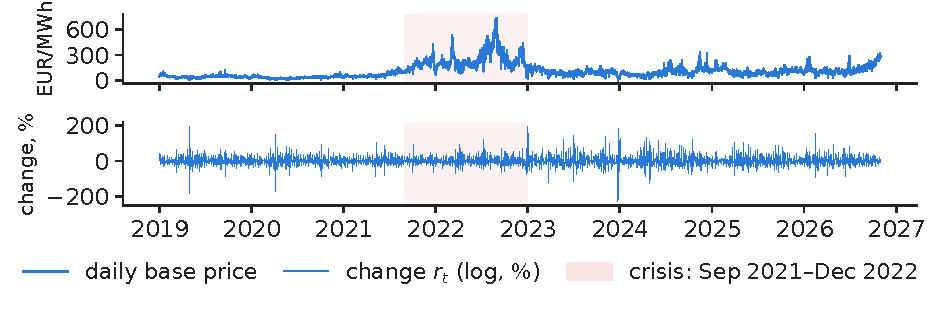
\includegraphics[width=\textwidth,height=0.487\textheight,keepaspectratio]{charts/en/returns_ro.pdf}\end{center}\vspace{-3mm}
\chartsource{Source: energy-charts.info (Fraunhofer ISE); OPCOM day-ahead prices for Romania, via ENTSO-E. Data: daily, 2019-01-01 to 2026-10-31, CET delivery days.}
\vspace{0.5mm}
\begin{itemize}\setlength{\itemsep}{0pt}
  \item Extreme days
    \begin{itemize}\setlength{\itemsep}{0pt}
      \item Largest rise \ensuremath{+}194\% on 2 Jan 2023, largest fall \ensuremath{-}227\% on 25 Dec 2023 (Christmas)
      \item 189 days with $|r_t|>50\%$ out of 2\,860
    \end{itemize}
\end{itemize}
\par\vfill\manager{a calm month says little about next month: risk comes in clusters.}\par\vspace{0.5mm}
\par\vfill\noindent{\scriptsize\color{FooterGray}(OPCOM day-ahead prices)}\hfill\qlink{EMQA\_L3\_returns\_ro}{Quantlets/L3/EMQA_L3_returns_ro}\par\vspace{0.5mm}
\end{frame}

\begin{frame}{Near zero the percent change explodes; below zero it does not exist}
\footnotesize
\intuition{The logarithm needs positive prices; near zero, ordinary moves become huge percentages.}
\begin{columns}[T,onlytextwidth]
\begin{column}{0.52\textwidth}
\[ \operatorname{asinh}(x)=\ln\bigl(x+\sqrt{x^2+1}\bigr) \]\vspace{-2mm}\[ \Delta\operatorname{asinh}P_t\approx\Delta\ln P_t\ \ \text{if}\ P_t\gg 1 \]{\footnotesize\begin{itemize}\setlength{\itemsep}{0pt}
  \item \textbf{\txtwhere}
    \begin{itemize}\setlength{\itemsep}{0pt}
      \item $\operatorname{asinh}$ = inverse hyperbolic sine, defined for any sign
      \item From 100 to 120 EUR/MWh both formulas give 18.2\%
      \item Near zero both explode.
    \end{itemize}
\end{itemize}\par}
\end{column}
\begin{column}{0.45\textwidth}
\begin{itemize}\setlength{\itemsep}{1pt}
  \item \textbf{On our data}, 2019--2026
    \begin{itemize}\setlength{\itemsep}{0pt}
      \item Romania: base price always positive (minimum 3.97 EUR/MWh)
      \item But 485 hours with negative prices, on 117 days
      \item DE-LU: 20 days with base price $\le 0$; from 0.95 to 92.91 EUR/MWh: $r_t$ = 458\%
    \end{itemize}
  \item \textbf{Our choice}
    \begin{itemize}\setlength{\itemsep}{0pt}
      \item Base price: $r_t$ (\%) and $\Delta P_t$ (EUR/MWh); hourly prices: EUR/MWh
    \end{itemize}
\end{itemize}
\end{column}
\end{columns}
\par\vfill\manager{a position is in MWh, so its risk is in EUR/MWh
    \begin{itemize}\setlength{\itemsep}{0pt}
      \item Use percent only far from zero.
    \end{itemize}}\par\vspace{0.5mm}
\par\vfill\noindent{\scriptsize\color{FooterGray}(Uniejewski, Weron \& Ziel, 2018, IEEE TPWRS)}\hfill\tryit{notebook \S1}\par\vspace{0.5mm}
\end{frame}

\begin{frame}{Half of the daily change is the weekly calendar, known in advance}
\small
\vspace{-1mm}\[ r_t=c+\textstyle\sum_{k=1}^{7}\phi_k r_{t-k}+\sum_{j=2}^{7}\delta_j D_{j,t}+\varepsilon_t \]\vspace{-2mm}
\begin{center}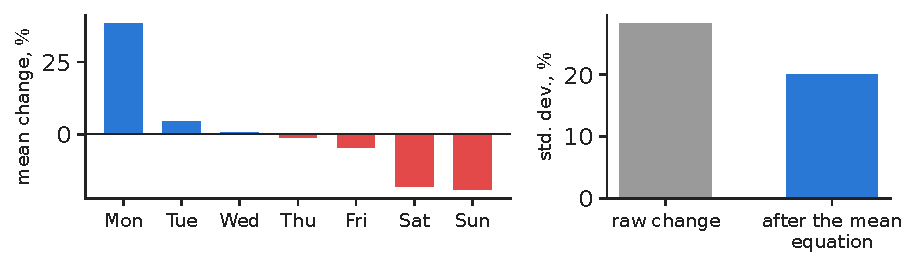
\includegraphics[width=\textwidth,height=0.400\textheight,keepaspectratio]{charts/en/dow_effect.pdf}\end{center}\vspace{-3mm}
\chartsource{Source: energy-charts.info (Fraunhofer ISE); OPCOM day-ahead prices for Romania, via ENTSO-E. Data: daily, 2019-01-01 to 2026-10-31.}
\vspace{0.5mm}
\begin{itemize}\setlength{\itemsep}{0pt}
  \item Mean equation: $\phi_k$ = weight of the change $k$ days ago, $D_{j,t}=1$ if day $t$ is weekday $j$; $R^2$ = 0.50
    \begin{itemize}\setlength{\itemsep}{0pt}
      \item Standard deviation 28.3\% before, 20.0\% after; models below use $\varepsilon_t$ and, in EUR/MWh, $u_t$
    \end{itemize}
\end{itemize}
\par\vfill\manager{a Monday price jump is not a risk signal: forecast it, do not hedge it.}\par\vspace{0.5mm}
\par\vfill\noindent{\scriptsize\color{FooterGray}(own estimation; Weron, 2014, IJF)}\hfill\qlink{EMQA\_L3\_dow\_effect}{Quantlets/L3/EMQA_L3_dow_effect}\par\vspace{0.5mm}
\end{frame}

\subsection{Stylised facts}

\begin{frame}{The sign of a shock is unpredictable, its size is not}
\small
\begin{center}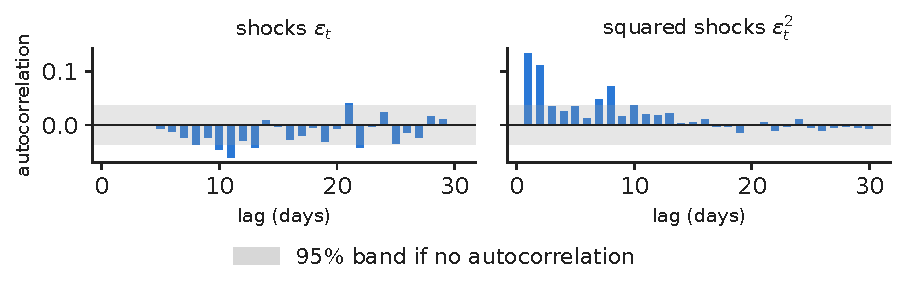
\includegraphics[width=\textwidth,height=0.418\textheight,keepaspectratio]{charts/en/acf_clust.pdf}\end{center}\vspace{-3mm}
\chartsource{Source: energy-charts.info (Fraunhofer ISE); OPCOM day-ahead prices for Romania, via ENTSO-E. Data: residuals of the mean equation, 2019-01-01 to 2026-10-31.}
\vspace{0.5mm}
\begin{itemize}\setlength{\itemsep}{0pt}
  \item Ljung--Box $Q(10)=T(T+2)\sum_{k\le10}\hat\rho_k^2/(T-k)$, $\hat\rho_k$ = autocorrelation at lag $k$: 13.8 for $\varepsilon_t$ ($p$ = 0.18), 120.0 for $\varepsilon_t^2$ (critical value 18.31)
    \begin{itemize}\setlength{\itemsep}{0pt}
      \item Lagrange multiplier test for autoregressive conditional heteroskedasticity (ARCH-LM), 10 lags: 93.7, $p<0.001$
    \end{itemize}
\end{itemize}
\par\vfill\manager{a large shock today announces large shocks in the next days: the subject of this lecture.}\par\vspace{0.5mm}
\par\vfill\noindent{\scriptsize\color{FooterGray}(Ljung \& Box, 1978; Engle, 1982, Econometrica)}\hfill\qlink{EMQA\_L3\_acf\_clust}{Quantlets/L3/EMQA_L3_acf_clust}\par\vspace{0.5mm}
\end{frame}

\begin{frame}{Extreme days are far more frequent than the normal law allows}
\small
\begin{center}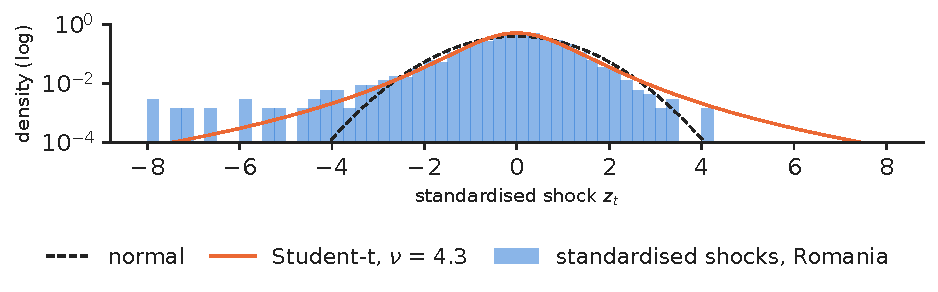
\includegraphics[width=\textwidth,height=0.475\textheight,keepaspectratio]{charts/en/tails.pdf}\end{center}\vspace{-3mm}
\chartsource{Source: energy-charts.info (OPCOM, via ENTSO-E); own estimates. Data: GARCH(1,1)-t on percent changes, 2019-01-01 to 2026-10-31.}
\vspace{0.5mm}
\begin{itemize}\setlength{\itemsep}{0pt}
  \item Shocks $\varepsilon_t$: excess kurtosis 20.0, skewness \ensuremath{-}1.69 (large falls: holidays, windy days)
    \begin{itemize}\setlength{\itemsep}{0pt}
      \item 15 shocks beyond 4 standard deviations, against 0.18 expected under normality; Student-t with $\nu$ = 4.3 degrees of freedom
    \end{itemize}
\end{itemize}
\par\vfill\manager{a limit built on the normal curve is breached far more often than planned (Lecture 4).}\par\vspace{0.5mm}
\par\vfill\noindent{\scriptsize\color{FooterGray}(own estimation; Bollerslev, 1987, RESTAT)}\hfill\qlink{EMQA\_L3\_tails}{Quantlets/L3/EMQA_L3_tails}\par\vspace{0.5mm}
\end{frame}

\begin{frame}{The crisis: same volatility in percent, 4 times higher in EUR/MWh}
\small
\begin{center}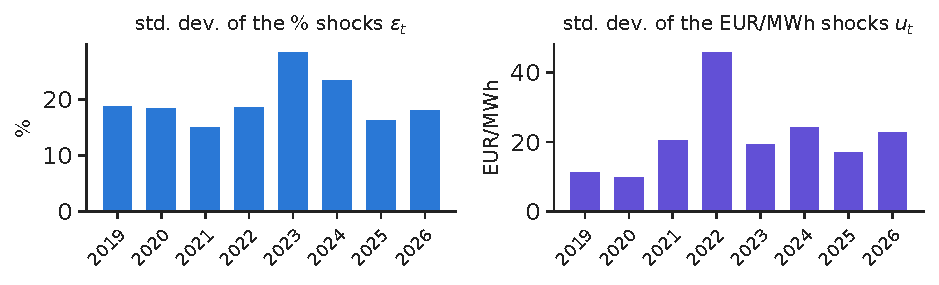
\includegraphics[width=\textwidth,height=0.477\textheight,keepaspectratio]{charts/en/vol_units.pdf}\end{center}\vspace{-3mm}
\chartsource{Source: energy-charts.info (Fraunhofer ISE); OPCOM day-ahead prices for Romania, via ENTSO-E. Data: residuals of the mean equation, 2019-01-01 to 2026-10-31.}
\vspace{0.5mm}
\begin{itemize}\setlength{\itemsep}{0pt}
  \item Standard deviation of the shocks, 2019 vs 2022
    \begin{itemize}\setlength{\itemsep}{0pt}
      \item In percent: 18.7\% vs 18.5\% (ratio 0.99)
      \item In EUR/MWh: 11.2 vs 45.8 (ratio 4.1); mean price 50 vs 265 EUR/MWh
    \end{itemize}
\end{itemize}
\par\vfill\manager{margin calls are paid in EUR: collateral rose with the price level although percent volatility did not.}\par\vspace{0.5mm}
\par\vfill\noindent{\scriptsize\color{FooterGray}(own estimation)}\hfill\qlink{EMQA\_L3\_vol\_units}{Quantlets/L3/EMQA_L3_vol_units}\par\vspace{0.5mm}
\end{frame}

\begin{frame}{Power prices are about 9 times more volatile than oil}
\footnotesize
\begin{center}{\footnotesize\renewcommand{\arraystretch}{1.05}\setlength{\tabcolsep}{4pt}
\begin{tabular}{@{}lrrrrrrrr@{}}\toprule
Annualised volatility, \% & 2019 & 2020 & 2021 & 2022 & 2023 & 2024 & 2025 & 2026 \\ \midrule
Power, Romania & \cellcolor{Crimson!43}358 & \cellcolor{Crimson!41}349 & \cellcolor{Crimson!23}287 & \cellcolor{Crimson!42}354 & \cellcolor{Crimson!55}543 & \cellcolor{Crimson!55}444 & \cellcolor{Crimson!29}310 & \cellcolor{Crimson!40}346 \\
Power, Hungary & \cellcolor{Crimson!12}247 & \cellcolor{Crimson!35}329 & \cellcolor{Crimson!23}289 & \cellcolor{Crimson!37}335 & \cellcolor{Crimson!55}566 & \cellcolor{Crimson!55}547 & \cellcolor{Crimson!43}358 & \cellcolor{Crimson!38}339 \\
EUA & -- & -- & -- & \cellcolor{Forest!44}53 & \cellcolor{Forest!50}32 & \cellcolor{Forest!48}37 & \cellcolor{Forest!52}24 & \cellcolor{Forest!51}28 \\
Brent & \cellcolor{Forest!50}30 & \cellcolor{Forest!39}71 & \cellcolor{Forest!50}32 & \cellcolor{Forest!46}46 & \cellcolor{Forest!50}31 & \cellcolor{Forest!52}25 & \cellcolor{Forest!50}29 & \cellcolor{Forest!43}56 \\
TTF gas (monthly) & \cellcolor{Forest!47}42 & \cellcolor{Forest!35}82 & \cellcolor{Forest!42}58 & \cellcolor{Forest!30}100 & \cellcolor{Forest!37}78 & \cellcolor{Forest!48}38 & \cellcolor{Forest!51}28 & \cellcolor{Forest!41}63 \\
OMV Petrom (SNP) & \cellcolor{Forest!52}24 & \cellcolor{Forest!49}35 & \cellcolor{Forest!52}22 & \cellcolor{Forest!52}22 & \cellcolor{Forest!54}18 & \cellcolor{Forest!54}17 & \cellcolor{Forest!53}20 & \cellcolor{Forest!53}21 \\
Hidroelectrica (H2O) & -- & -- & -- & -- & \cellcolor{Forest!55}13 & \cellcolor{Forest!55}14 & \cellcolor{Forest!55}14 & \cellcolor{Forest!50}30 \\
\bottomrule\end{tabular}}\end{center}\vspace{-1mm}\begin{itemize}\setlength{\itemsep}{1pt}
  \item \textbf{How to read it}
    \begin{itemize}\setlength{\itemsep}{0pt}
      \item Daily shocks: standard deviation $\times\sqrt{365}$ for power, $\times\sqrt{252}$ for traded assets; TTF: monthly averages $\times\sqrt{12}$ (understates risk)
      \item Brent peaks in 2020 and 2026, carbon in 2022; -- = series not yet available
    \end{itemize}
\end{itemize}
\par\vfill\manager{never compare the limits of a power desk with those of an oil desk in the same percent.}\par\vspace{0.5mm}
\par\vfill\noindent{\scriptsize\color{FooterGray}(own estimation; World Bank Pink Sheet)}\hfill\tryit{notebook \S2}\par\vspace{0.5mm}
\end{frame}


\section{The GARCH family}

\subsection{GARCH(1,1) and its estimation}

\begin{frame}{GARCH updates tomorrow's variance from today's shock}
\footnotesize
\intuition{A big shock yesterday raises today's variance; the effect then fades day by day.}
\begin{columns}[T,onlytextwidth]
\begin{column}{0.58\textwidth}
\[ \sigma_t^2=\underbrace{\omega}_{\text{constant}}+\underbrace{\alpha\,\varepsilon_{t-1}^2}_{\text{reaction to the shock}}+\underbrace{\beta\,\sigma_{t-1}^2}_{\text{memory}} \]\vspace{-1mm}\[ \varepsilon_t=\sigma_t z_t,\qquad \bar\sigma^2=\frac{\omega}{1-\alpha-\beta} \]{\footnotesize\begin{itemize}\setlength{\itemsep}{0pt}
  \item \textbf{\txtwhere}
    \begin{itemize}\setlength{\itemsep}{0pt}
      \item $\sigma_t^2$ = conditional variance, known on the evening of $t-1$
      \item $z_t$ = standardised shock (mean 0, variance 1)
      \item $\omega>0$, $\alpha,\beta\ge0$, persistence $\alpha+\beta<1$, long-run variance $\bar\sigma^2$
      \item $\beta=0$: ARCH model (Engle, 1982).
    \end{itemize}
\end{itemize}\par}
\end{column}
\begin{column}{0.39\textwidth}
\begin{itemize}\setlength{\itemsep}{1pt}
  \item \textbf{Romania, shocks in \%}
    \begin{itemize}\setlength{\itemsep}{0pt}
      \item $\hat\alpha$ = 0.308, $\hat\beta$ = 0.438, $\hat\alpha+\hat\beta$ = 0.746
      \item Long-run $\bar\sigma$ = 20.4\% per day
    \end{itemize}
  \item \textbf{Romania, shocks in EUR/MWh}
    \begin{itemize}\setlength{\itemsep}{0pt}
      \item $\hat\alpha$ = 0.102, $\hat\beta$ = 0.892, $\hat\alpha+\hat\beta$ = 0.994
      \item Long-run $\bar\sigma$ = 27.6 EUR/MWh per day
    \end{itemize}
\end{itemize}
\end{column}
\end{columns}
\par\vfill\manager{every evening GARCH gives the risk desk tomorrow's $\sigma$, from data it already has.}\par\vspace{0.5mm}
\par\vfill\noindent{\scriptsize\color{FooterGray}(Engle, 1982, Econometrica; Bollerslev, 1986, JOE)}\hfill\tryit{notebook \S3}\par\vspace{0.5mm}
\end{frame}

\begin{frame}{Parameters are estimated by maximum likelihood with Student-t shocks}
\footnotesize
\intuition{Choose the parameters that make the observed shocks most probable; Student-t leaves room for extreme days.}
\begin{columns}[T,onlytextwidth]
\begin{column}{0.50\textwidth}
\[ \ell(\omega,\alpha,\beta,\nu)=\sum_{t=1}^{T}\Bigl[\ln f_\nu\Bigl(\frac{\varepsilon_t}{\sigma_t}\Bigr)-\ln\sigma_t\Bigr] \]{\footnotesize\begin{itemize}\setlength{\itemsep}{0pt}
  \item \textbf{\txtwhere}
    \begin{itemize}\setlength{\itemsep}{0pt}
      \item $f_\nu$ = Student-t density with variance 1 and $\nu>2$ degrees of freedom
      \item Small $\nu$ = fat tails, $\nu\to\infty$ = normal
      \item Bayesian information criterion (BIC) $=k\ln T-2\hat\ell$, $k$ = number of parameters (lower = better)
      \item Appendix A.
    \end{itemize}
\end{itemize}\par}
\end{column}
\begin{column}{0.47\textwidth}
{\footnotesize\renewcommand{\arraystretch}{1.15}\setlength{\tabcolsep}{4pt}
\begin{tabular}{@{}lrr@{}}\toprule
GARCH(1,1), shocks in \% & normal & Student \\ \midrule
log-likelihood & \ensuremath{-}12\,360.3 & \ensuremath{-}12\,094.5 \\
BIC & 24\,744.5 & 24\,220.8 \\
$\hat\alpha+\hat\beta$ & 0.927 & 0.746 \\
half-life, days & 9.2 & 2.4 \\
$\hat\nu$ & -- & 4.27 \\
\bottomrule\end{tabular}}\begin{itemize}\setlength{\itemsep}{1pt}
  \item \textbf{Reading}
    \begin{itemize}\setlength{\itemsep}{0pt}
      \item Student wins (lower BIC); the normal model reads every holiday as lasting volatility
    \end{itemize}
\end{itemize}
\end{column}
\end{columns}
\par\vfill\manager{use Student-t shocks
    \begin{itemize}\setlength{\itemsep}{0pt}
      \item With normal shocks the limits stay wide for too long.
    \end{itemize}}\par\vspace{0.5mm}
\par\vfill\noindent{\scriptsize\color{FooterGray}(Bollerslev, 1987, RESTAT)}\hfill\tryit{notebook \S3}\par\vspace{0.5mm}
\end{frame}

\begin{frame}{GARCH volatility: short spikes in percent, a long hump in EUR/MWh}
\small
\begin{center}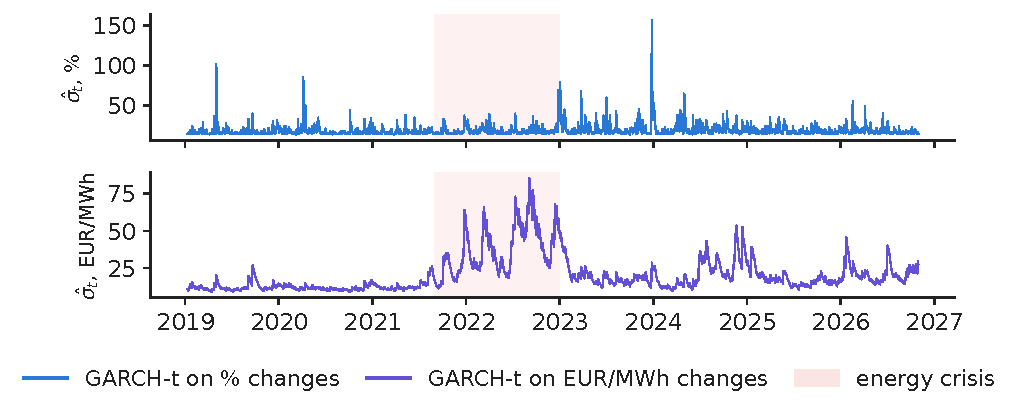
\includegraphics[width=\textwidth,height=0.516\textheight,keepaspectratio]{charts/en/cond_vol.pdf}\end{center}\vspace{-3mm}
\chartsource{Source: energy-charts.info (OPCOM, via ENTSO-E); own estimates. Data: GARCH(1,1)-t, 2019-01-01 to 2026-10-31.}
\vspace{0.5mm}
\begin{itemize}\setlength{\itemsep}{0pt}
  \item Peaks
    \begin{itemize}\setlength{\itemsep}{0pt}
      \item In percent: 156\% per day on 26 Dec 2023, gone within days
      \item In EUR/MWh: 85.7 on 4 Sep 2022, against a minimum of 8.8 on 6 Jul 2019; 27.4 at the cut-off
    \end{itemize}
\end{itemize}
\par\vfill\manager{a supplier's collateral follows the EUR/MWh line, not the percent line.}\par\vspace{0.5mm}
\par\vfill\noindent{\scriptsize\color{FooterGray}(own estimation, GARCH(1,1)-t)}\hfill\qlink{EMQA\_L3\_cond\_vol}{Quantlets/L3/EMQA_L3_cond_vol}\par\vspace{0.5mm}
\end{frame}

\subsection{Persistence and half-life}

\begin{frame}{The half-life counts the days until half of a volatility shock is gone}
\footnotesize
\intuition{The extra variance created by a shock shrinks every day by the factor $\alpha+\beta$.}
\begin{columns}[T,onlytextwidth]
\begin{column}{0.49\textwidth}
\[ \E_t\bigl[\sigma^2_{t+h}\bigr]-\bar\sigma^2=(\alpha+\beta)^{h-1}\bigl(\sigma^2_{t+1}-\bar\sigma^2\bigr) \]\vspace{-1mm}\[ h_{1/2}=\frac{\ln 0.5}{\ln(\alpha+\beta)} \]{\footnotesize\begin{itemize}\setlength{\itemsep}{0pt}
  \item \textbf{\txtwhere}
    \begin{itemize}\setlength{\itemsep}{0pt}
      \item $\E_t$ = expectation given the data up to day $t$
      \item $h$ = days ahead
      \item $h_{1/2}$ = half-life
      \item Derivation in Appendix B.
    \end{itemize}
\end{itemize}\par}
\end{column}
\begin{column}{0.48\textwidth}
{\footnotesize\renewcommand{\arraystretch}{1.12}\setlength{\tabcolsep}{4pt}
\begin{tabular}{@{}lrrl@{}}\toprule
GARCH(1,1)-t & $\hat\alpha+\hat\beta$ & $h_{1/2}$ & unit \\ \midrule
Romania, \% & 0.746 & 2.4 & days \\
Romania, EUR/MWh & 0.994 & 113.5 & days \\
Hungary, \% & 0.881 & 5.5 & days \\
Brent & 0.973 & 25.6 & trading days \\
EUA & 0.992 & 82.8 & trading days \\
OMV Petrom & 0.934 & 10.2 & trading days \\
\bottomrule\end{tabular}}
\par\vspace{0.5mm}{\scriptsize \begin{itemize}\setlength{\itemsep}{0pt}
  \item Samples: power and Brent from 2019, EUA from 19 Oct 2021, OMV Petrom from 2019.
\end{itemize}}
\end{column}
\end{columns}
\par\vfill\manager{after an oil shock keep wider limits for about 5 weeks
    \begin{itemize}\setlength{\itemsep}{0pt}
      \item After a percent shock in power, for days.
    \end{itemize}}\par\vspace{0.5mm}
\par\vfill\noindent{\scriptsize\color{FooterGray}(Engle, 2001, JEP)}\hfill\tryit{notebook \S3}\par\vspace{0.5mm}
\end{frame}

\begin{frame}{Answer to Lecture 1: oil and carbon shocks fade in weeks, not days}
\small
\begin{center}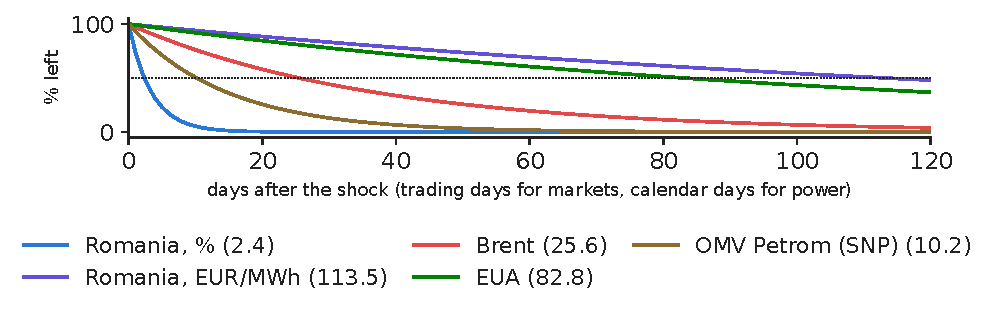
\includegraphics[width=\textwidth,height=0.470\textheight,keepaspectratio]{charts/en/halflife.pdf}\end{center}\vspace{-3mm}
\chartsource{Source: energy-charts.info (OPCOM, via ENTSO-E); Yahoo Finance (Brent BZ=F, SparkChange EUA ETC); EODHD (BVB shares). Data: GARCH(1,1)-t, each series over its own sample (table on the slide).}
\vspace{0.5mm}
\begin{itemize}\setlength{\itemsep}{0pt}
  \item Curves: $100(\hat\alpha+\hat\beta)^h$ = percent of the extra variance left after $h$ days; half-lives in brackets
    \begin{itemize}\setlength{\itemsep}{0pt}
      \item Brent 26 trading days, about 5 weeks; EUA 83, about 17 weeks
      \item Romania: 2.4 days in percent, but 114 days in EUR/MWh, because volatility in money follows the price level
    \end{itemize}
\end{itemize}
\par\vfill\manager{after a shock, a risk desk keeps wider limits for weeks, not days, as announced in Lecture 1.}\par\vspace{0.5mm}
\par\vfill\noindent{\scriptsize\color{FooterGray}(own estimation)}\hfill\qlink{EMQA\_L3\_halflife}{Quantlets/L3/EMQA_L3_halflife}\par\vspace{0.5mm}
\end{frame}

\subsection{Asymmetry}

\begin{frame}{Asymmetric GARCH: rises and falls do not move volatility equally}
\footnotesize
\intuition{Two extensions let a rise and a fall of the same size have different effects on tomorrow's variance.}
\begin{columns}[T,onlytextwidth]
\begin{column}{0.52\textwidth}
\[ \text{GJR:}\ \ \sigma_t^2=\omega+(\alpha+\gamma I_{t-1})\varepsilon_{t-1}^2+\beta\sigma_{t-1}^2 \]\[ \text{EGARCH:}\ \ \ln\sigma_t^2=\omega+\alpha\bigl(|z_{t-1}|-\sqrt{2/\pi}\bigr)+\gamma z_{t-1}+\beta\ln\sigma_{t-1}^2 \]{\footnotesize\begin{itemize}\setlength{\itemsep}{0pt}
  \item \textbf{\txtwhere}
    \begin{itemize}\setlength{\itemsep}{0pt}
      \item $I_{t-1}=1$ if $\varepsilon_{t-1}<0$, else 0
      \item Glosten--Jagannathan--Runkle (GJR): $\gamma>0$ = falls raise volatility more (leverage effect of shares), $\gamma<0$ = rises do
      \item Exponential GARCH (EGARCH): opposite sign convention for $\gamma$.
    \end{itemize}
\end{itemize}\par}
\end{column}
\begin{column}{0.45\textwidth}
\begin{itemize}\setlength{\itemsep}{1pt}
  \item \textbf{Romania, shocks in \%}
    \begin{itemize}\setlength{\itemsep}{0pt}
      \item GJR: $\hat\gamma$ = 0.225 ($t$ = 2.9); EGARCH: $\hat\gamma$ = \ensuremath{-}0.083 ($t$ = \ensuremath{-}3.9)
      \item Falls raise volatility more (rebound after a drop)
    \end{itemize}
  \item \textbf{Romania, shocks in EUR/MWh}
    \begin{itemize}\setlength{\itemsep}{0pt}
      \item GJR: $\hat\gamma$ = \ensuremath{-}0.127 ($t$ = \ensuremath{-}6.4); EGARCH: $\hat\gamma$ = 0.104 ($t$ = 7.2)
      \item Rises raise volatility more: inverse leverage effect
    \end{itemize}
\end{itemize}
\end{column}
\end{columns}
\par\vfill\manager{for a buyer the dangerous direction is up: after a price jump, widen the limits more than after a fall.}\par\vspace{0.5mm}
\par\vfill\noindent{\scriptsize\color{FooterGray}(Glosten et al., 1993, JFIN; Nelson, 1991; Knittel \& Roberts, 2005, ENEECO)}\hfill\tryit{notebook \S4}\par\vspace{0.5mm}
\end{frame}

\begin{frame}{In EUR/MWh, rises raise volatility more: the inverse leverage effect}
\small
\begin{center}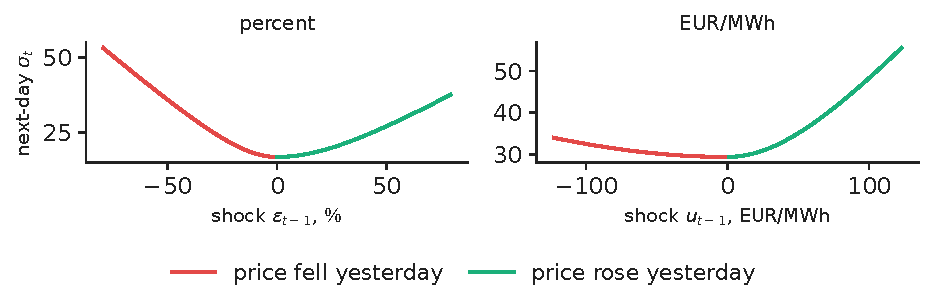
\includegraphics[width=\textwidth,height=0.500\textheight,keepaspectratio]{charts/en/nic.pdf}\end{center}\vspace{-3mm}
\chartsource{Source: energy-charts.info (OPCOM, via ENTSO-E); own estimates. Data: GJR(1,1)-t, 2019-01-01 to 2026-10-31.}
\vspace{0.5mm}
\begin{itemize}\setlength{\itemsep}{0pt}
  \item News impact curve: next-day $\sigma$ as a function of today's shock (GJR); for a shock of 61 EUR/MWh
    \begin{itemize}\setlength{\itemsep}{0pt}
      \item Next-day $\sigma$ = 37.6 EUR/MWh after a rise, 30.6 after a fall
      \item In percent (shock of 40\%) the order is reversed: 30.3\% after a fall, 23.7\% after a rise
    \end{itemize}
\end{itemize}
\par\vfill\manager{an industrial consumer on spot prices should react faster to rises than to falls.}\par\vspace{0.5mm}
\par\vfill\noindent{\scriptsize\color{FooterGray}(Engle \& Ng, 1993, JFIN; own estimation, GJR(1,1)-t)}\hfill\qlink{EMQA\_L3\_nic}{Quantlets/L3/EMQA_L3_nic}\par\vspace{0.5mm}
\end{frame}

\begin{frame}{Volatility in EUR/MWh grows with the price level}
\small
\begin{center}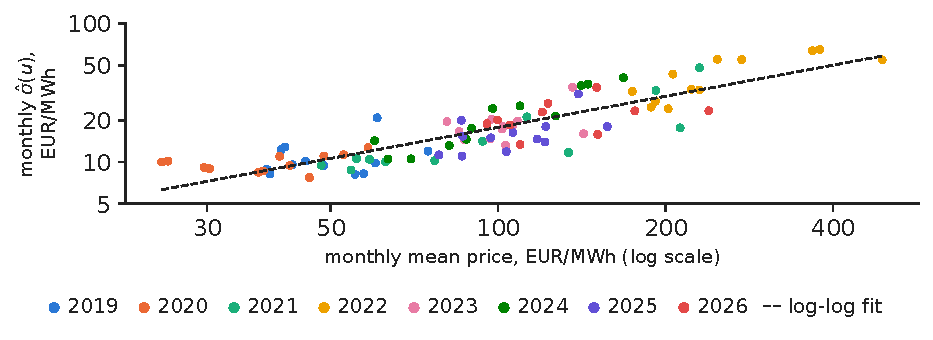
\includegraphics[width=\textwidth,height=0.480\textheight,keepaspectratio]{charts/en/vol_level.pdf}\end{center}\vspace{-3mm}
\chartsource{Source: energy-charts.info (Fraunhofer ISE); OPCOM day-ahead prices for Romania, via ENTSO-E. Data: monthly, 2019-01-01 to 2026-10-31.}
\vspace{0.5mm}
\begin{itemize}\setlength{\itemsep}{0pt}
  \item Why: at high prices the supply curve (merit order) is steeper, so the same demand shock moves the price more
    \begin{itemize}\setlength{\itemsep}{0pt}
      \item Regression of $\ln\hat\sigma_m(u)$ on $\ln\bar P_m$, 94 months: slope 0.75, $R^2$ = 0.76; in percent: slope 0.01, $R^2$ = 0.00
    \end{itemize}
\end{itemize}
\par\vfill\manager{set EUR/MWh limits as a share of the forward price, not as a fixed amount.}\par\vspace{0.5mm}
\par\vfill\noindent{\scriptsize\color{FooterGray}(Knittel \& Roberts, 2005, ENEECO; own estimation)}\hfill\qlink{EMQA\_L3\_vol\_level}{Quantlets/L3/EMQA_L3_vol_level}\par\vspace{0.5mm}
\end{frame}

\begin{frame}{Fat tails matter more than asymmetry}
\footnotesize
\begin{center}{\footnotesize\renewcommand{\arraystretch}{1.05}\setlength{\tabcolsep}{4pt}
\begin{tabular}{@{}lrrrrrr@{}}\toprule
Model & $\alpha+\beta$ (\%) & BIC (\%) & $p$, $z^2$ (\%) & $\alpha+\beta$ (EUR) & BIC (EUR) & $p$, $z^2$ (EUR) \\ \midrule
GARCH, normal & 0.927 & \cellcolor{Crimson!55}24\,744.5 & 0.328 & 0.998 & \cellcolor{Crimson!55}24\,573.2 & 0.000 \\
GARCH, Student & 0.746 & \cellcolor{Forest!54}24\,220.8 & 0.367 & 0.994 & \cellcolor{Forest!25}24\,450.7 & 0.000 \\
GJR, normal & 0.651 & \cellcolor{Crimson!44}24\,690.7 & 0.151 & 0.998 & \cellcolor{Crimson!24}24\,525.1 & 0.000 \\
GJR, Student & 0.727 & \cellcolor{Forest!55}24\,214.1 & 0.243 & 0.996 & \cellcolor{Forest!50}24\,411.7 & 0.000 \\
EGARCH, normal & 0.903 & \cellcolor{Crimson!44}24\,691.4 & 0.529 & 0.995 & \cellcolor{Crimson!19}24\,518.0 & 0.000 \\
EGARCH, Student & 0.831 & \cellcolor{Forest!54}24\,219.2 & 0.532 & 0.995 & \cellcolor{Forest!55}24\,403.9 & 0.000 \\
\bottomrule\end{tabular}}\end{center}\vspace{-1mm}\begin{itemize}\setlength{\itemsep}{1pt}
  \item \textbf{Ranking by BIC} (green = best)
    \begin{itemize}\setlength{\itemsep}{0pt}
      \item Every Student-t model beats every normal one; best: GJR-t in \%, EGARCH-t in EUR/MWh; Akaike information criterion (AIC) in Appendix C
    \end{itemize}
  \item \textbf{Diagnostic}: Ljung--Box $p$ for $z_t^2$, the squared standardised shocks
    \begin{itemize}\setlength{\itemsep}{0pt}
      \item In \% no clustering is left; in EUR/MWh some is ($p<0.001$): one equation cannot follow both the price level and the daily shocks
    \end{itemize}
\end{itemize}
\par\vfill\manager{first get the tails right, then worry about asymmetry.}\par\vspace{0.5mm}
\par\vfill\noindent{\scriptsize\color{FooterGray}(Bollerslev, 1987; Glosten, Jagannathan \& Runkle, 1993; Nelson, 1991)}\hfill\tryit{notebook \S4}\par\vspace{0.5mm}
\end{frame}


\section{Regimes and the energy crisis}

\begin{frame}{A Markov-switching model separates calm and turbulent regimes}
\footnotesize
\intuition{Two hidden states, each with its own volatility; for every day the model gives the probability of the turbulent one.}
\begin{columns}[T,onlytextwidth]
\begin{column}{0.52\textwidth}
\[ u_t=\mu_{s_t}+\sigma_{s_t}\eta_t,\qquad \Pr(s_t=j\mid s_{t-1}=i)=p_{ij} \]\vspace{-1mm}\[ \text{expected duration of regime } i=\frac{1}{1-p_{ii}} \]{\footnotesize\begin{itemize}\setlength{\itemsep}{0pt}
  \item \textbf{\txtwhere}
    \begin{itemize}\setlength{\itemsep}{0pt}
      \item $u_t$ = shock in EUR/MWh
      \item $s_t$ = regime (calm or turbulent)
      \item $\eta_t$ = standard normal
      \item $p_{ij}$ = transition probabilities, by maximum likelihood (Appendix D).
    \end{itemize}
\end{itemize}\par}
\end{column}
\begin{column}{0.45\textwidth}
\begin{itemize}\setlength{\itemsep}{1pt}
  \item \textbf{Romania, shocks in EUR/MWh}
    \begin{itemize}\setlength{\itemsep}{0pt}
      \item Calm: $\sigma$ = 12.9, $p_{11}$ = 0.986, about 69 days
      \item Turbulent: $\sigma$ = 41.9, $p_{22}$ = 0.957, about 23 days; 24\% of all days
    \end{itemize}
  \item \textbf{In percent}
    \begin{itemize}\setlength{\itemsep}{0pt}
      \item Turbulent state: only 3.5 days, isolated spikes
    \end{itemize}
\end{itemize}
\end{column}
\end{columns}
\par\vfill\manager{a turbulent-regime probability above 0.5 triggers a review of hedges and collateral.}\par\vspace{0.5mm}
\par\vfill\noindent{\scriptsize\color{FooterGray}(Hamilton, 1989, Econometrica)}\hfill\tryit{notebook \S5}\par\vspace{0.5mm}
\end{frame}

\begin{frame}{The crisis was one long turbulent regime; 2026 moves in and out}
\small
\begin{center}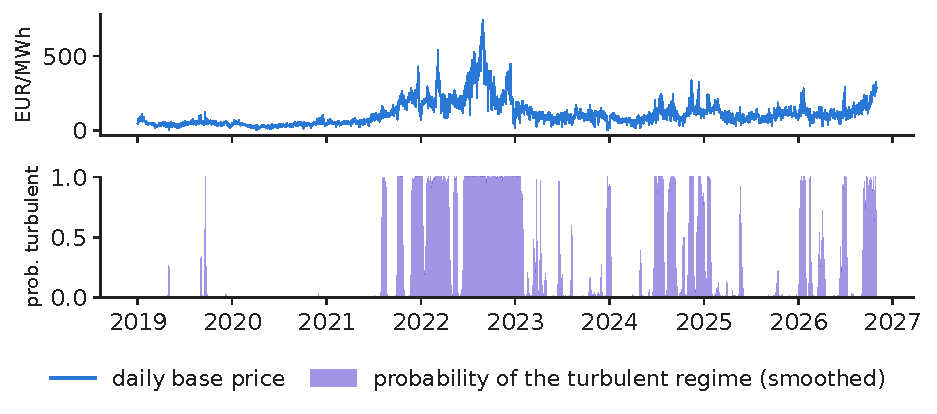
\includegraphics[width=\textwidth,height=0.485\textheight,keepaspectratio]{charts/en/ms_regime.pdf}\end{center}\vspace{-3mm}
\chartsource{Source: energy-charts.info (OPCOM, via ENTSO-E); own estimates. Data: two-regime Markov-switching model on EUR/MWh shocks, 2019-01-01 to 2026-10-31.}
\vspace{0.5mm}
\begin{itemize}\setlength{\itemsep}{0pt}
  \item Turbulent days
    \begin{itemize}\setlength{\itemsep}{0pt}
      \item Longest spell: 15 Jun 2022 -- 31 Jan 2023, 231 days
      \item Share by year: 2022 86\%, 2025 6\%, 2026 33\% (48\% since July)
    \end{itemize}
\end{itemize}
\par\vfill\manager{Transelectrica and suppliers can use the regime probability as an early warning for balancing costs.}\par\vspace{0.5mm}
\par\vfill\noindent{\scriptsize\color{FooterGray}(own estimation; Hamilton, 1989)}\hfill\qlink{EMQA\_L3\_ms\_regime}{Quantlets/L3/EMQA_L3_ms_regime}\par\vspace{0.5mm}
\end{frame}

\begin{frame}{Persistence depends on the period and on the unit}
\footnotesize
\begin{center}{\footnotesize\renewcommand{\arraystretch}{1.1}\setlength{\tabcolsep}{4pt}
\begin{tabular}{@{}lrrrrr@{}}\toprule
GARCH(1,1)-t on & $\hat\alpha+\hat\beta$ (\%) & $h_{1/2}$ (\%) & $\hat\alpha+\hat\beta$ (EUR) & $h_{1/2}$ (EUR) & $\bar\sigma$, EUR/MWh \\ \midrule
2019--2020 (calm) & 0.568 & 1.2 & 0.208 & 0.4 & 10.5 \\
2021--2022 (crisis) & 0.882 & 5.5 & 1.000 & $\infty$ & -- \\
2023 -- Oct 2026 & 0.727 & 2.2 & 0.927 & 9.1 & 20.9 \\
whole sample & 0.746 & 2.4 & 0.994 & 113.5 & 27.6 \\
\bottomrule\end{tabular}}\end{center}\vspace{-1mm}\begin{itemize}\setlength{\itemsep}{1pt}
  \item \textbf{In EUR/MWh}
    \begin{itemize}\setlength{\itemsep}{0pt}
      \item In 2019--2020 a shock halves in under a day; in the crisis $\hat\alpha+\hat\beta$ reaches 1, because volatility rose with the price month after month
      \item The whole-sample value mixes regimes, and mixing regimes overstates persistence
    \end{itemize}
  \item \textbf{In percent}
    \begin{itemize}\setlength{\itemsep}{0pt}
      \item Persistence stays well below 1 in every period: the crisis moved the level, not percent volatility
    \end{itemize}
\end{itemize}
\par\vfill\manager{re-estimate after a regime change
    \begin{itemize}\setlength{\itemsep}{0pt}
      \item A model fitted on the crisis keeps limits wide for too long.
    \end{itemize}}\par\vspace{0.5mm}
\par\vfill\noindent{\scriptsize\color{FooterGray}(Lamoureux \& Lastrapes, 1990, JBES; own estimation)}\hfill\tryit{notebook \S5}\par\vspace{0.5mm}
\end{frame}


\section{Intraday volatility from hourly prices}

\begin{frame}{Intraday variation measures how much the price moves within a day}
\footnotesize
\intuition{Sum the squared hour-to-hour changes of one delivery day; this is the variation a battery or a flexible consumer earns from.}
\begin{columns}[T,onlytextwidth]
\begin{column}{0.52\textwidth}
\[ \text{RV}_d=\sqrt{\textstyle\sum_{h=1}^{H_d-1}\bigl(P_{d,h}-P_{d,h-1}\bigr)^2},\qquad \text{relative}=\frac{\text{RV}_d}{\bar P_d} \]{\footnotesize\begin{itemize}\setlength{\itemsep}{0pt}
  \item \textbf{\txtwhere}
    \begin{itemize}\setlength{\itemsep}{0pt}
      \item $P_{d,h}$ = price of hour $h$ of day $d$ (from 1 October 2025, mean of the four quarter-hours)
      \item $H_d$ = 24 hours (23 or 25 on the 8 + 8 clock-change days)
      \item $\bar P_d$ = daily base price
      \item In EUR/MWh, because hourly prices can be negative.
    \end{itemize}
\end{itemize}\par}
\end{column}
\begin{column}{0.45\textwidth}
\begin{itemize}\setlength{\itemsep}{1pt}
  \item \textbf{Realised intraday variation (RV)}, yearly mean
    \begin{itemize}\setlength{\itemsep}{0pt}
      \item 2019: 36; 2022: 186; 2026: 135 EUR/MWh
      \item Relative to the price (median): 0.64 in 2019, 1.24 in 2024
    \end{itemize}
  \item \textbf{A different risk}
    \begin{itemize}\setlength{\itemsep}{0pt}
      \item Correlation between RV$_d$ and $|u_t|$: only 0.46
      \item Not the realised volatility of finance: the 24 hours are 24 different products
    \end{itemize}
\end{itemize}
\end{column}
\end{columns}
\par\vfill\manager{a battery developer's revenue scales with intraday variation, not with the daily average price.}\par\vspace{0.5mm}
\par\vfill\noindent{\scriptsize\color{FooterGray}(Andersen \& Bollerslev, 1998, IER; Weron, 2014, IJF)}\hfill\tryit{notebook \S6}\par\vspace{0.5mm}
\end{frame}

\begin{frame}{Solar generation has made the price move more within the day}
\small
\begin{center}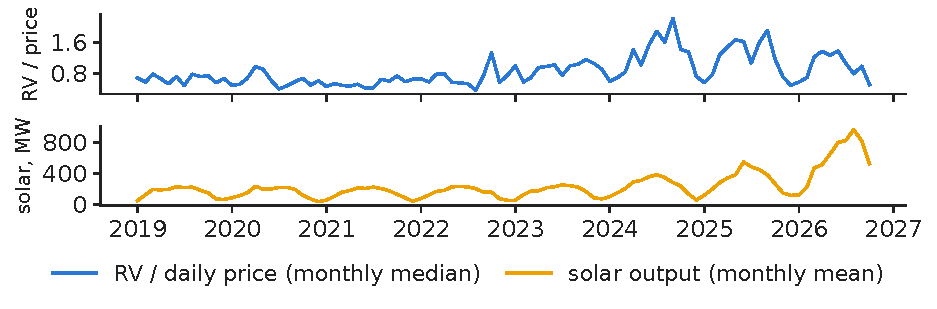
\includegraphics[width=\textwidth,height=0.487\textheight,keepaspectratio]{charts/en/rv_solar.pdf}\end{center}\vspace{-3mm}
\chartsource{Source: energy-charts.info (Fraunhofer ISE); OPCOM prices; ENTSO-E solar generation (Transelectrica data for Romania). Data: hourly prices, monthly values, 2019-01-01 to 2026-10-31.}
\vspace{0.5mm}
\begin{itemize}\setlength{\itemsep}{0pt}
  \item Relative intraday variation (median)
    \begin{itemize}\setlength{\itemsep}{0pt}
      \item 0.64 in 2019, peak 1.24 in 2024, 1.01 in 2026
      \item Mean solar output: 157 MW in 2019, 593 MW in Jan -- Oct 2026; monthly correlation 0.46
    \end{itemize}
\end{itemize}
\par\vfill\manager{more solar means cheaper middays and dearer evenings: the business case of storage.}\par\vspace{0.5mm}
\par\vfill\noindent{\scriptsize\color{FooterGray}(own estimation; ENTSO-E solar generation)}\hfill\qlink{EMQA\_L3\_rv\_solar}{Quantlets/L3/EMQA_L3_rv_solar}\par\vspace{0.5mm}
\end{frame}

\begin{frame}{Intraday variation has a long memory: day, week and month}
\footnotesize
\intuition{Three averages over different horizons give a simple long-memory regression.}
\begin{columns}[T,onlytextwidth]
\begin{column}{0.56\textwidth}
\[ \begin{aligned}\ln\text{RV}_d=b_0&+b_D\ln\text{RV}_{d-1}+\tfrac{b_W}{7}\textstyle\sum_{j=1}^{7}\ln\text{RV}_{d-j}\\ &+\tfrac{b_M}{30}\textstyle\sum_{j=1}^{30}\ln\text{RV}_{d-j}+e_d\end{aligned} \]{\footnotesize\begin{itemize}\setlength{\itemsep}{0pt}
  \item \textbf{\txtwhere}
    \begin{itemize}\setlength{\itemsep}{0pt}
      \item Heterogeneous autoregressive (HAR) model, by ordinary least squares (OLS)
      \item $b_D$, $b_W$, $b_M$ = weights of yesterday, the last 7 and 30 days
      \item Forecast $=\exp(\widehat{\ln\text{RV}}_d+s^2/2)$, $s^2$ = residual variance.
    \end{itemize}
\end{itemize}\par}
\end{column}
\begin{column}{0.41\textwidth}
\begin{itemize}\setlength{\itemsep}{1pt}
  \item \textbf{Estimates}, before the test year
    \begin{itemize}\setlength{\itemsep}{0pt}
      \item $\hat b_D$ = 0.40, $\hat b_W$ = 0.36, $\hat b_M$ = 0.22 (all $t>$ 6), $R^2$ = 0.82
    \end{itemize}
  \item \textbf{Test year}
    \begin{itemize}\setlength{\itemsep}{0pt}
      \item Mean absolute error (MAE): HAR 35.6, yesterday's value 39.1 EUR/MWh (9.1\% less)
    \end{itemize}
\end{itemize}
\end{column}
\end{columns}
\par\vfill\manager{a battery operator schedules maintenance on days with low forecast variation.}\par\vspace{0.5mm}
\par\vfill\noindent{\scriptsize\color{FooterGray}(Corsi, 2009, JFEC)}\hfill\tryit{notebook \S6}\par\vspace{0.5mm}
\end{frame}

\begin{frame}{HAR forecasts follow intraday variation, not its isolated spikes}
\small
\begin{center}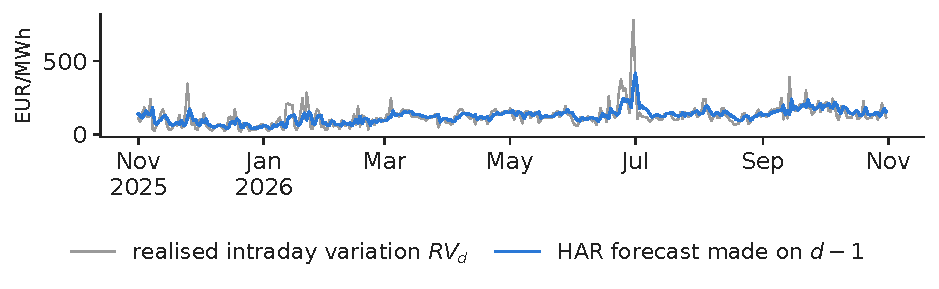
\includegraphics[width=\textwidth,height=0.470\textheight,keepaspectratio]{charts/en/har_fc.pdf}\end{center}\vspace{-3mm}
\chartsource{Source: energy-charts.info (Fraunhofer ISE); OPCOM day-ahead prices for Romania, via ENTSO-E. Data: test year 2025-11-01 to 2026-10-31; HAR re-estimated daily.}
\vspace{0.5mm}
\begin{itemize}\setlength{\itemsep}{0pt}
  \item Test year, forecast made on $d-1$
    \begin{itemize}\setlength{\itemsep}{0pt}
      \item HAR re-estimated every day on the data available on $d-1$; MAE 35.6 EUR/MWh
    \end{itemize}
\end{itemize}
\par\vfill\manager{use the forecast for planning
    \begin{itemize}\setlength{\itemsep}{0pt}
      \item Keep reserves for the spikes it cannot see.
    \end{itemize}}\par\vspace{0.5mm}
\par\vfill\noindent{\scriptsize\color{FooterGray}(own estimation)}\hfill\qlink{EMQA\_L3\_har\_fc}{Quantlets/L3/EMQA_L3_har_fc}\par\vspace{0.5mm}
\end{frame}


\section{Forecasting and evaluating volatility}

\begin{frame}{A volatility forecast is judged against a noisy proxy}
\footnotesize
\intuition{We compare the forecast with a noisy proxy, the squared shock, using a loss that still ranks models correctly.}
\begin{columns}[T,onlytextwidth]
\begin{column}{0.52\textwidth}
\[ \text{QLIKE}_t=\frac{\varepsilon_t^2}{\hat\sigma_t^2}-\ln\frac{\varepsilon_t^2}{\hat\sigma_t^2}-1,\qquad \text{MSE}_t=\bigl(\varepsilon_t^2-\hat\sigma_t^2\bigr)^2 \]{\footnotesize\begin{itemize}\setlength{\itemsep}{0pt}
  \item \textbf{\txtwhere}
    \begin{itemize}\setlength{\itemsep}{0pt}
      \item Quasi-likelihood loss (QLIKE), mean squared error (MSE)
      \item $\varepsilon_t$ = out-of-sample shock of day $t$
      \item $\hat\sigma_t^2$ = forecast made on $t-1$
      \item MSE is dominated by a few extreme days
      \item Diebold--Mariano (DM) test on the daily loss differences.
    \end{itemize}
\end{itemize}\par}
\end{column}
\begin{column}{0.45\textwidth}
\begin{itemize}\setlength{\itemsep}{1pt}
  \item \textbf{Example}: true $\sigma$ = 20
    \begin{itemize}\setlength{\itemsep}{0pt}
      \item Forecast 10: QLIKE = 1.61; forecast 40: QLIKE = 0.64
      \item Underestimating costs 2.5 times more; MSE says the opposite
    \end{itemize}
  \item \textbf{Design}, test year 1 Nov 2025 -- 31 Oct 2026
    \begin{itemize}\setlength{\itemsep}{0pt}
      \item Five models re-estimated daily on data up to $t-1$
    \end{itemize}
\end{itemize}
\end{column}
\end{columns}
\par\vfill\manager{ask your risk vendor for QLIKE on your own days, out of sample.}\par\vspace{0.5mm}
\par\vfill\noindent{\scriptsize\color{FooterGray}(Patton, 2011, JOE; Hansen \& Lunde, 2005, JAE)}\hfill\tryit{notebook \S7}\par\vspace{0.5mm}
\end{frame}

\begin{frame}{GARCH-type forecasts beat the 30-day history, significantly in EUR}
\footnotesize
\begin{center}{\footnotesize\renewcommand{\arraystretch}{1.05}\setlength{\tabcolsep}{4pt}
\begin{tabular}{@{}lrrrr@{}}\toprule
One-day-ahead variance & QLIKE, \% & $p$ vs 30-day & QLIKE, EUR & $p$ vs 30-day \\ \midrule
30-day historical variance & \cellcolor{Crimson!55}1.523 & -- & \cellcolor{Crimson!55}1.428 & -- \\
exponentially weighted average (EWMA) & \cellcolor{Crimson!21}1.499 & 0.082 & \cellcolor{Crimson!13}1.398 & 0.026 \\
GARCH(1,1)-t & \cellcolor{Forest!35}1.459 & 0.170 & \cellcolor{Forest!15}1.378 & 0.040 \\
GJR(1,1)-t & \cellcolor{Forest!55}1.445 & 0.145 & \cellcolor{Forest!44}1.357 & 0.032 \\
EGARCH(1,1)-t & \cellcolor{Forest!45}1.452 & 0.120 & \cellcolor{Forest!55}1.349 & 0.027 \\
\bottomrule\end{tabular}}\end{center}\vspace{-1mm}\begin{itemize}\setlength{\itemsep}{1pt}
  \item \textbf{Reading}
    \begin{itemize}\setlength{\itemsep}{0pt}
      \item Lower QLIKE = better (green); $p$ = one-sided DM test (Newey--West, 7 lags), 365 days
      \item Best: GJR-t in \% (5.1\% below the 30-day loss), EGARCH-t in EUR/MWh (5.5\%)
    \end{itemize}
  \item \textbf{Significance at 5\%}
    \begin{itemize}\setlength{\itemsep}{0pt}
      \item EUR/MWh: all GARCH-type models beat the history; percent: none does; asymmetry adds nothing significant ($p$ = 0.08)
    \end{itemize}
\end{itemize}
\par\vfill\manager{use GARCH-t as the default
    \begin{itemize}\setlength{\itemsep}{0pt}
      \item Asymmetric models add little out of sample.
    \end{itemize}}\par\vspace{0.5mm}
\par\vfill\noindent{\scriptsize\color{FooterGray}(Diebold \& Mariano, 1995, JBES; Patton, 2011, JOE; RiskMetrics, 1996)}\hfill\tryit{notebook \S7}\par\vspace{0.5mm}
\end{frame}

\begin{frame}{GARCH reacts at once; the 30-day history lags, then forgets abruptly}
\small
\begin{center}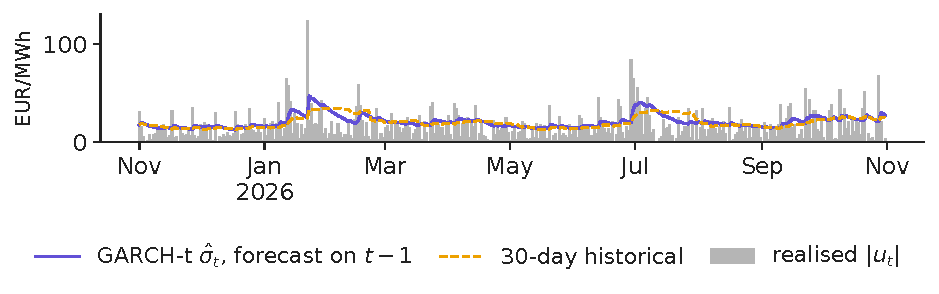
\includegraphics[width=\textwidth,height=0.451\textheight,keepaspectratio]{charts/en/fc_test.pdf}\end{center}\vspace{-3mm}
\chartsource{Source: energy-charts.info (OPCOM, via ENTSO-E); own estimates. Data: test year 2025-11-01 to 2026-10-31; models re-estimated daily.}
\vspace{0.5mm}
\begin{itemize}\setlength{\itemsep}{0pt}
  \item Largest shock of the test year: \ensuremath{+}124 EUR/MWh on 22 Jan 2026
    \begin{itemize}\setlength{\itemsep}{0pt}
      \item Next day: GARCH $\hat\sigma$ from 25 to 47, history only 33 EUR/MWh
      \item 30 days later the shock leaves the window: the history drops from 32 to 23 overnight
    \end{itemize}
\end{itemize}
\par\vfill\manager{a limit that jumps 30 days after a shock, with no news, is a warning sign of a historical-window model.}\par\vspace{0.5mm}
\par\vfill\noindent{\scriptsize\color{FooterGray}(own estimation, test year 1 Nov 2025 -- 31 Oct 2026)}\hfill\qlink{EMQA\_L3\_fc\_test}{Quantlets/L3/EMQA_L3_fc_test}\par\vspace{0.5mm}
\end{frame}

\begin{frame}{Weeks ahead, volatility returns to its long-run level}
\footnotesize
\intuition{High volatility is expected to fall and low volatility to rise, so $\sigma\sqrt{h}$ misstates the risk over $h$ days.}
\begin{columns}[T,onlytextwidth]
\begin{column}{0.52\textwidth}
\[ \hat\sigma^2_{T+h\mid T}=\bar\sigma^2+(\alpha+\beta)^{h-1}\bigl(\hat\sigma^2_{T+1}-\bar\sigma^2\bigr) \]\vspace{-1mm}\[ \Var_T\Bigl(\textstyle\sum_{k=1}^{h}r_{T+k}\Bigr)=\sum_{k=1}^{h}\hat\sigma^2_{T+k\mid T}\ \ne\ h\,\hat\sigma^2_{T+1} \]{\footnotesize\begin{itemize}\setlength{\itemsep}{0pt}
  \item \textbf{\txtwhere}
    \begin{itemize}\setlength{\itemsep}{0pt}
      \item $T$ = forecast day
      \item Second formula: returns without autocorrelation (oil, carbon), not power
      \item 90\% band = $\pm1.645\sqrt{\cdot}$.
    \end{itemize}
\end{itemize}\par}
\end{column}
\begin{column}{0.45\textwidth}
\begin{itemize}\setlength{\itemsep}{1pt}
  \item \textbf{Brent on 9 Apr 2026}, after the 2026 oil shock
    \begin{itemize}\setlength{\itemsep}{0pt}
      \item $\hat\sigma_{T+1}$ = 93\% a year, long-run 39\%
      \item 20-day band: GARCH $\pm$38.5\%, $\sigma\sqrt{20}$ $\pm$43.1\% (12\% too wide)
    \end{itemize}
  \item \textbf{Brent on 30 Oct 2026}, calm again
    \begin{itemize}\setlength{\itemsep}{0pt}
      \item $\hat\sigma_{T+1}$ = 32\% $<$ 40\%: now $\sigma\sqrt{20}$ is too narrow
    \end{itemize}
\end{itemize}
\end{column}
\end{columns}
\par\vfill\manager{an industrial buyer budgeting next month's fuel should add the GARCH forecasts, not scale today's $\sigma$.}\par\vspace{0.5mm}
\par\vfill\noindent{\scriptsize\color{FooterGray}(Engle, 2001, JEP; own estimation)}\hfill\tryit{notebook \S7}\par\vspace{0.5mm}
\end{frame}


\section{Case study: Romanian power in 2026}

\begin{frame}{Case study: 2026 is a level shock, not (yet) a new 2022}
\footnotesize
\begin{itemize}\setlength{\itemsep}{1pt}
  \item \textbf{What happened to prices}
    \begin{itemize}\setlength{\itemsep}{0pt}
      \item Romanian base price: 150 EUR/MWh in January, 239 in October 2026 (monthly means)
      \item Brent: 69 USD/bbl in February, 100 in March, 108 in October; TTF gas: 32 $\to$ 87 EUR/MWh (February $\to$ October)
    \end{itemize}
  \item \textbf{What happened to volatility}
    \begin{itemize}\setlength{\itemsep}{0pt}
      \item In percent, nothing: mean monthly $\hat\sigma$ 17.4\% in 2026, 17.4\% in 2022, 16.6\% in 2019
      \item In EUR/MWh it doubled from 2019 (10.9 $\to$ 21.8), but its peak month, 34.7 (Jan 2026), stays far below 2022 (65.1, Sep 2022)
      \item Turbulent regime: 33\% of the days of 2026 (2022: 86\%); probability 0.47 on 31 Oct 2026
      \item Brent: GARCH volatility up to 100\% annualised (9 Apr 2026), against 30\% on average in 2025
    \end{itemize}
  \item \textbf{Verdict}
    \begin{itemize}\setlength{\itemsep}{0pt}
      \item A shock to the price level, with a turbulent regime about half of the time since July; not (yet) a 2022
    \end{itemize}
\end{itemize}
\par\vfill\manager{a supplier renewing contracts in November 2026 should price risk on the higher level, not on a new volatility regime.}\par\vspace{0.5mm}
\par\vfill\noindent{\scriptsize\color{FooterGray}(own estimation; World Bank Pink Sheet; Yahoo Finance)}\hfill\tryit{notebook \S8}\par\vspace{0.5mm}
\end{frame}

\begin{frame}{Case study: the one-day GARCH-t band held over the test year}
\small
\begin{center}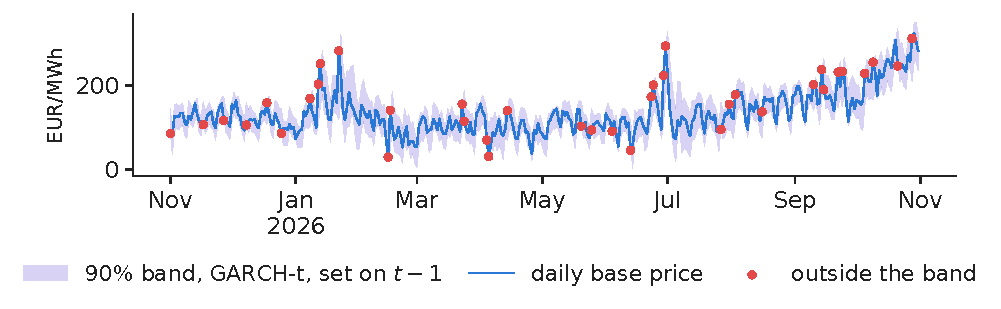
\includegraphics[width=\textwidth,height=0.464\textheight,keepaspectratio]{charts/en/case_band.pdf}\end{center}\vspace{-3mm}
\chartsource{Source: energy-charts.info (OPCOM, via ENTSO-E); own estimates. Data: test year 2025-11-01 to 2026-10-31.}
\vspace{0.5mm}
\begin{itemize}\setlength{\itemsep}{0pt}
  \item Band = forecast price $\pm$ Student quantile $\times\hat\sigma_t$, set on $t-1$
    \begin{itemize}\setlength{\itemsep}{0pt}
      \item 38 of 365 days outside (10.4\%, 10\% expected): 9.4\% from November to April, 11.4\% from May to October
      \item Mean half-width 33 EUR/MWh in the first half, 36 in September--October
    \end{itemize}
\end{itemize}
\par\vfill\manager{a supplier can set its daily purchase limit from this band
    \begin{itemize}\setlength{\itemsep}{0pt}
      \item The formal tests of such bands come in Lecture 4.
    \end{itemize}}\par\vspace{0.5mm}
\par\vfill\noindent{\scriptsize\color{FooterGray}(own estimation, test year 1 Nov 2025 -- 31 Oct 2026)}\hfill\qlink{EMQA\_L3\_case\_band}{Quantlets/L3/EMQA_L3_case_band}\par\vspace{0.5mm}
\end{frame}

\begin{frame}{Case study: November 2026 limits and the April oil shock}
\small
\begin{center}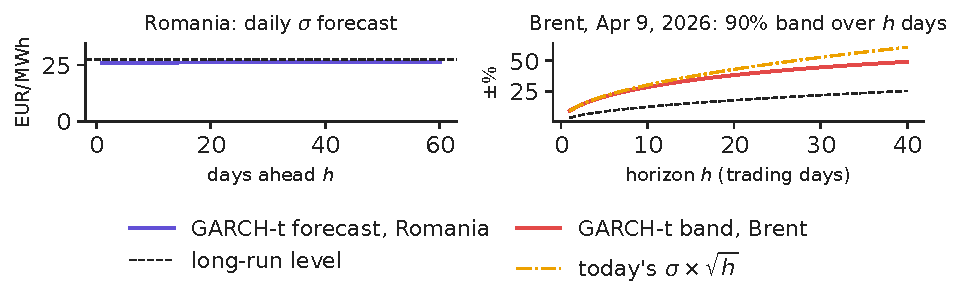
\includegraphics[width=\textwidth,height=0.500\textheight,keepaspectratio]{charts/en/term_structure.pdf}\end{center}\vspace{-3mm}
\chartsource{Source: energy-charts.info (OPCOM, via ENTSO-E); Yahoo Finance (Brent BZ=F, SparkChange EUA ETC); EODHD (BVB shares). Data: GARCH(1,1)-t forecasts made with data up to 2026-10-31.}
\vspace{0.5mm}
\begin{itemize}\setlength{\itemsep}{0pt}
  \item Romania, 31 Oct 2026: $\hat\sigma$ = 26.0 EUR/MWh, close to the long-run 27.6
    \begin{itemize}\setlength{\itemsep}{0pt}
      \item One-day 90\% limit about $\pm$43 EUR/MWh for each day of November; Brent: the band grows slower than $\sigma\sqrt{h}$
    \end{itemize}
\end{itemize}
\par\vfill\manager{set limits from the forecast term structure, not from today's volatility.}\par\vspace{0.5mm}
\par\vfill\noindent{\scriptsize\color{FooterGray}(own estimation)}\hfill\qlink{EMQA\_L3\_term\_structure}{Quantlets/L3/EMQA_L3_term_structure}\par\vspace{0.5mm}
\end{frame}

\begin{frame}{Case study C3: Romanian energy shares are weakly tied to oil}
\footnotesize
\begin{itemize}\setlength{\itemsep}{1pt}
  \item \textbf{What the paper did} (Grecu, Cramer, Pele \& Lessmann, 2025)
    \begin{itemize}\setlength{\itemsep}{0pt}
      \item Data: stock indices of the 27 European Union countries, Brent and TTF futures, 2010--2023
      \item Method: GARCH volatility for each series, then a dynamic conditional correlation (DCC) for each day; a Markov model for regimes of that correlation
      \item Result: the correlation with oil is mostly between 0 and 0.4; Central and Eastern Europe (CEE) is the least correlated region; regimes persist above 98\%
    \end{itemize}
  \item \textbf{Our replication} (OMV Petrom, Romgaz (SNG), Nuclearelectrica (SNN) vs Brent, 2\,860 days)
    \begin{itemize}\setlength{\itemsep}{0pt}
      \item DCC parameters $a$ = 0.021, $b$ = 0.950: a slow, very persistent correlation
      \item Mean correlation 0.13; maximum 0.54 in 2020, minimum \ensuremath{-}0.32 in 2022: the calendar of the paper
      \item Hedging the basket with Brent, out of sample: variance change \ensuremath{-}1.7\% (dynamic), \ensuremath{-}6.9\% (static); negative = more risk
    \end{itemize}
\end{itemize}
\par\vspace{0.5mm}{\scriptsize \begin{itemize}\setlength{\itemsep}{0pt}
  \item C3 numbers are computed by the C3 case notebook on our data; the paper's own results are in the case brief.
\end{itemize}}
\par\vfill\manager{the risk of Romanian energy shares is regulatory and local
    \begin{itemize}\setlength{\itemsep}{0pt}
      \item A Brent hedge does not reduce it.
    \end{itemize}}\par\vspace{0.5mm}
\par\vfill\noindent{\scriptsize\color{FooterGray}(Grecu, Cramer, Pele \& Lessmann, 2025, NAJEF; case study C3)}\par\vspace{0.5mm}
\end{frame}

\section*{Wrap-up}

\begin{frame}{Quiz 1: half-life of an oil shock}
\small
\begin{itemize}
  \item For Brent, GARCH(1,1)-t gives $\hat\alpha+\hat\beta$ = 0.973
    \begin{itemize}\setlength{\itemsep}{0pt}
      \item After a shock, how long until half of the extra variance is gone?
    \end{itemize}
\end{itemize}
\vspace{2mm}
\begin{exampleblock}{Answer}
\begin{itemize}
  \item $h_{1/2}=\ln 0.5/\ln$ 0.973 = 25.6 trading days, about 5 weeks: limits stay wider for weeks, not days.
\end{itemize}
\end{exampleblock}
\end{frame}

\begin{frame}{Quiz 2: percent or euro}
\small
\begin{itemize}
  \item In 2022 the percent volatility of the Romanian price was the same as in 2019
    \begin{itemize}\setlength{\itemsep}{0pt}
      \item Did the risk of a supplier's open position of 10 MW change?
    \end{itemize}
\end{itemize}
\vspace{2mm}
\begin{exampleblock}{Answer}
\begin{itemize}
  \item Yes: the position loses or gains in EUR, and the EUR/MWh volatility of the shocks rose 4.1 times, with the price level.
\end{itemize}
\end{exampleblock}
\end{frame}

\begin{frame}{Quiz 3: a Monday jump}
\small
\begin{itemize}
  \item The PZU price rises by 35\% from Sunday to Monday
    \begin{itemize}\setlength{\itemsep}{0pt}
      \item Should the risk desk widen the limits?
    \end{itemize}
\end{itemize}
\vspace{2mm}
\begin{exampleblock}{Answer}
\begin{itemize}
  \item No: on average Monday is \ensuremath{+}38\% above Sunday
    \begin{itemize}\setlength{\itemsep}{0pt}
      \item The calendar is forecast by the mean equation, and only the shock $\varepsilon_t$ (here almost zero) enters GARCH.
    \end{itemize}
\end{itemize}
\end{exampleblock}
\end{frame}

\begin{frame}{Quiz 4: choosing a volatility model}
\small
\begin{itemize}
  \item A vendor's volatility model has the lowest mean squared error on your test year, thanks to three extreme days
    \begin{itemize}\setlength{\itemsep}{0pt}
      \item What do you ask for?
    \end{itemize}
\end{itemize}
\vspace{2mm}
\begin{exampleblock}{Answer}
\begin{itemize}
  \item QLIKE on the same days and a DM test against GARCH-t and the 30-day history
    \begin{itemize}\setlength{\itemsep}{0pt}
      \item On our test year the best QLIKE in EUR/MWh is EGARCH-t, not significantly better than GARCH-t.
    \end{itemize}
\end{itemize}
\end{exampleblock}
\end{frame}

\begin{frame}{Quiz 5: after a rise or after a fall}
\small
\begin{itemize}
  \item Yesterday the price moved by 61 EUR/MWh
    \begin{itemize}\setlength{\itemsep}{0pt}
      \item For a buyer, is tomorrow riskier if it was a rise or a fall?
    \end{itemize}
\end{itemize}
\vspace{2mm}
\begin{exampleblock}{Answer}
\begin{itemize}
  \item After a rise: the GJR model in EUR/MWh gives $\sigma$ = 37.6 after a rise, 30.6 after a fall (inverse leverage effect).
\end{itemize}
\end{exampleblock}
\end{frame}

\begin{frame}{Wrap-up}
\small
\vspace{-2mm}\begin{multicols}{2}\scriptsize\tableofcontents[hideallsubsections]\end{multicols}
\begin{itemize}\setlength{\itemsep}{1pt}
  \item \textbf{Measure}
    \begin{itemize}\setlength{\itemsep}{0pt}
      \item Remove the weekly calendar first; in percent the crisis was not more volatile, in EUR/MWh it was 4.1 times more
    \end{itemize}
  \item \textbf{Model and forecast}
    \begin{itemize}\setlength{\itemsep}{0pt}
      \item GARCH-t is the default; oil shocks halve in about 5 weeks; next: risk measures for energy companies (Lecture 4)
    \end{itemize}
\end{itemize}
\end{frame}

\begin{frame}{Research from our group on volatility and risk}
\footnotesize
\begin{itemize}\setlength{\itemsep}{1pt}
  \item \textbf{Energy prices and EU stock markets} (Grecu, Cramer, Pele \& Lessmann, 2025, NAJEF)
    \begin{itemize}\setlength{\itemsep}{0pt}
      \item What it did: GARCH volatility, daily DCC correlations and Markov regimes for 27 national indices against oil and gas, 2010--2023
      \item Result: European markets follow oil more than gas, with persistent regimes (case study C3)
    \end{itemize}
  \item \textbf{Entropy and market risk} (Pele, Lazar \& Dufour, 2017, Entropy)
    \begin{itemize}\setlength{\itemsep}{0pt}
      \item What it did: measured the entropy of intraday euro--yen returns and related it to intraday value at risk (VaR) and expected shortfall (ES)
      \item Result: a negative relation between entropy and intraday VaR and ES; intraday entropy is then used to forecast the daily VaR
    \end{itemize}
  \item \textbf{High-frequency entropy for daily risk} (Pele \& Mazurencu-Marinescu-Pele, 2019, Entropy)
    \begin{itemize}\setlength{\itemsep}{0pt}
      \item What it did: used the entropy of intraday Bitcoin returns to forecast the daily VaR, against classical GARCH models
      \item Result: the entropy-based VaR forecast performs best in the backtests: intraday data carry information on daily risk
    \end{itemize}
  \item \textbf{Energy Financial Risk Meter} (Toma, Dima, Grecu, Pele \& Lessmann, 2026, SSRN)
    \begin{itemize}\setlength{\itemsep}{0pt}
      \item What it did: a systemic-risk indicator for the EU energy sector; preview of Lecture 4
    \end{itemize}
\end{itemize}
\par\vspace{0.5mm}{\scriptsize \begin{itemize}\setlength{\itemsep}{0pt}
  \item Findings as stated in the papers; numbers on the other slides come from our own data.
\end{itemize}}
\par\vfill\noindent{\scriptsize\color{FooterGray}(Bucharest University of Economic Studies; Romanian Academy, Institute for Economic Forecasting)}\par\vspace{0.5mm}
\end{frame}

\begin{frame}{AIDA 2026: geopolitical crises turn the energy link of EU stocks negative}
\footnotesize
\begin{itemize}\setlength{\itemsep}{1pt}
  \item \textbf{What the work did} (A.-A.\ Cramer, AIDA (AI and Digital Assets in Energy and Finance) conference, 3 June 2026)
    \begin{itemize}\setlength{\itemsep}{0pt}
      \item Data: main stock index of each EU country, by region and by industrialisation; Brent and TTF futures, 2010--2026
      \item Models: GARCH, then a daily DCC correlation (as in case study C3); Markov regimes; responses to shocks
    \end{itemize}
  \item \textbf{What it found}
    \begin{itemize}\setlength{\itemsep}{0pt}
      \item Correlation with oil mostly positive, in most cases between 0 and 0.4; with gas generally lower than with oil
      \item Oil matters most in Southern and Western Europe, gas in the North and West; industrialised countries follow oil more
      \item Crises turn the correlation negative: Crimea 2014 (gas), Ukraine 2022 (gas: strongest in CEE), the Middle East 2026
      \item After a shock, the most industrialised countries are hit more in the first months, then the effect fades
    \end{itemize}
\end{itemize}
\par\vspace{0.5mm}{\scriptsize \begin{itemize}\setlength{\itemsep}{0pt}
  \item Findings as stated by the authors. Talk: \href{https://github.com/danpele/EMQA/blob/main/resources/aida2026/cramer_energy_stock_markets.pdf}{slides}; paper: \href{https://doi.org/10.1016/j.najef.2025.102420}{doi:10.1016/j.najef.2025.102420}.
\end{itemize}}
\par\vfill\manager{whoever hedges EU shares with oil or gas futures must expect the correlation to flip sign in a crisis.}\par\vspace{0.5mm}
\par\vfill\noindent{\scriptsize\color{FooterGray}(Cramer, AIDA conference, Bucharest, 3 June 2026; Grecu, Cramer, Pele \& Lessmann, 2025, NAJEF)}\par\vspace{0.5mm}
\end{frame}

\begin{frame}{AIDA 2026: spillovers of energy tokens are mostly short-run}
\footnotesize
\begin{itemize}\setlength{\itemsep}{1pt}
  \item \textbf{What the work did} (S.\ Ben Amor \& M.\ Horváth, AIDA conference, 4 June 2026)
    \begin{itemize}\setlength{\itemsep}{0pt}
      \item Data: energy tokens (Power Ledger, SunContract, Energy Web), cryptocurrencies, clean-energy stocks, oil, gas, carbon allowances, green bonds; Dec 2020 -- Jan 2026
      \item Model: a time-varying vector autoregression; spillovers split into short-run (transitory) and long-run (persistent) parts
    \end{itemize}
  \item \textbf{What it found}
    \begin{itemize}\setlength{\itemsep}{0pt}
      \item Connectedness: about 60\% of the total in the short run, about 5\% in the long run
      \item Crises (crypto turmoil 2021, energy crisis 2022) amplify short-run shocks; the long-run structure stays flat
      \item Power Ledger and SunContract are the main short-run transmitters; Energy Web matters mainly in stress episodes
      \item Diversification is token-specific: minimum-variance portfolio, Sharpe ratio 0.127 without tokens, 0.143 with SunContract
    \end{itemize}
\end{itemize}
\par\vspace{0.5mm}{\scriptsize \begin{itemize}\setlength{\itemsep}{0pt}
  \item Findings as stated by the authors. Talk: \href{https://github.com/danpele/EMQA/blob/main/resources/aida2026/benamor_energy_tokens_spillovers.pdf}{slides}.
\end{itemize}}
\par\vfill\manager{shocks pass within days
    \begin{itemize}\setlength{\itemsep}{0pt}
      \item Judge the diversification value token by token.
    \end{itemize}}\par\vspace{0.5mm}
\par\vfill\noindent{\scriptsize\color{FooterGray}(Ben Amor \& Horváth, AIDA conference, Bucharest, 4 June 2026)}\par\vspace{0.5mm}
\end{frame}

\begin{frame}{Want to learn more?}
\small
\begin{columns}[T,onlytextwidth]
\begin{column}{0.52\textwidth}
\begin{itemize}\setlength{\itemsep}{1pt}
  \item \textbf{R.\,F.\ Engle, GARCH 101} (2001): the clearest short introduction, by the Nobel laureate who invented ARCH --- \href{https://doi.org/10.1257/jep.15.4.157}{doi:10.1257/jep.15.4.157}.
  \item \textbf{R.\ Weron, Modeling and Forecasting Electricity Loads and Prices} (Wiley, 2006): stylised facts and volatility of power prices --- \href{https://doi.org/10.1002/9781118673362}{doi:10.1002/9781118673362}.
  \item \textbf{The \texttt{arch} Python package} (K.\ Sheppard), used for every model of this lecture: \href{https://arch.readthedocs.io}{arch.readthedocs.io}.
\end{itemize}
\end{column}
\begin{column}{0.45\textwidth}
\begin{itemize}\setlength{\itemsep}{1pt}
  \item \textbf{This course}: code, data, notebooks --- \href{https://github.com/danpele/EMQA}{github.com/danpele/EMQA}.
  \item \textbf{Case study C3}: the DCC model and the Brent hedge for Romanian energy shares, step by step.
  \item \textbf{Experiment yourself}: the notebook reproduces every chart and number of this lecture --- \href{\emqarepo/\emqanb}{notebooks/}.
\end{itemize}
\end{column}
\end{columns}
\end{frame}

\begin{frame}{References (1/3)}
\scriptsize
\begin{itemize}\setlength{\itemsep}{1pt}\scriptsize
\item Andersen, T.\,G.\ \& Bollerslev, T.\ (1998). Answering the skeptics: Yes, standard volatility models do provide accurate forecasts. \textit{International Economic Review}, 39(4), 885--905. \href{https://doi.org/10.2307/2527343}{doi:10.2307/2527343}
\item Ben Amor, S.\ \& Horváth, M.\ (2026). Transitory and persistent cross-market spillovers of energy tokens. AIDA Conference, Bucharest University of Economic Studies, 4 June 2026. \href{https://github.com/danpele/EMQA/blob/main/resources/aida2026/benamor_energy_tokens_spillovers.pdf}{github.com/danpele/EMQA/resources/aida2026}
\item Bollerslev, T.\ (1986). Generalized autoregressive conditional heteroskedasticity. \textit{Journal of Econometrics}, 31(3), 307--327. \href{https://doi.org/10.1016/0304-4076(86)90063-1}{doi:10.1016/0304-4076(86)90063-1}
\item Bollerslev, T.\ (1987). A conditionally heteroskedastic time series model for speculative prices and rates of return. \textit{Review of Economics and Statistics}, 69(3), 542--547. \href{https://doi.org/10.2307/1925546}{doi:10.2307/1925546}
\item Corsi, F.\ (2009). A simple approximate long-memory model of realized volatility. \textit{Journal of Financial Econometrics}, 7(2), 174--196. \href{https://doi.org/10.1093/jjfinec/nbp001}{doi:10.1093/jjfinec/nbp001}
\item Cramer, A.-A.\ (2026). The link between energy prices and stock markets in European Union countries (with R.-A.\ Grecu, D.\,T.\ Pele and S.\ Lessmann). AIDA Conference, Bucharest University of Economic Studies, 3 June 2026. \href{https://github.com/danpele/EMQA/blob/main/resources/aida2026/cramer_energy_stock_markets.pdf}{github.com/danpele/EMQA/resources/aida2026}
\item Diebold, F.\,X.\ \& Mariano, R.\,S.\ (1995). Comparing predictive accuracy. \textit{Journal of Business \& Economic Statistics}, 13(3), 253--263. \href{https://doi.org/10.1080/07350015.1995.10524599}{doi:10.1080/07350015.1995.10524599}
\item Engle, R.\,F.\ (1982). Autoregressive conditional heteroscedasticity with estimates of the variance of United Kingdom inflation. \textit{Econometrica}, 50(4), 987--1007. \href{https://doi.org/10.2307/1912773}{doi:10.2307/1912773}
\end{itemize}
\end{frame}

\begin{frame}{References (2/3)}
\scriptsize
\begin{itemize}\setlength{\itemsep}{1pt}\scriptsize
\item Engle, R.\,F.\ (2001). GARCH 101: The use of ARCH/GARCH models in applied econometrics. \textit{Journal of Economic Perspectives}, 15(4), 157--168. \href{https://doi.org/10.1257/jep.15.4.157}{doi:10.1257/jep.15.4.157}
\item Engle, R.\,F.\ \& Ng, V.\,K.\ (1993). Measuring and testing the impact of news on volatility. \textit{Journal of Finance}, 48(5), 1749--1778. \href{https://doi.org/10.1111/j.1540-6261.1993.tb05127.x}{doi:10.1111/j.1540-6261.1993.tb05127.x}
\item Glosten, L.\,R., Jagannathan, R.\ \& Runkle, D.\,E.\ (1993). On the relation between the expected value and the volatility of the nominal excess return on stocks. \textit{Journal of Finance}, 48(5), 1779--1801. \href{https://doi.org/10.1111/j.1540-6261.1993.tb05128.x}{doi:10.1111/j.1540-6261.1993.tb05128.x}
\item Grecu, R.\,A., Cramer, A.\,A., Pele, D.\,T.\ \& Lessmann, S.\ (2025). The link between energy prices and stock markets in European Union countries. \textit{North American Journal of Economics and Finance}, 78, 102420. \href{https://doi.org/10.1016/j.najef.2025.102420}{doi:10.1016/j.najef.2025.102420}
\item Hamilton, J.\,D.\ (1989). A new approach to the economic analysis of nonstationary time series and the business cycle. \textit{Econometrica}, 57(2), 357--384. \href{https://doi.org/10.2307/1912559}{doi:10.2307/1912559}
\item Hansen, P.\,R.\ \& Lunde, A.\ (2005). A forecast comparison of volatility models: Does anything beat a GARCH(1,1)? \textit{Journal of Applied Econometrics}, 20(7), 873--889. \href{https://doi.org/10.1002/jae.800}{doi:10.1002/jae.800}
\item Knittel, C.\,R.\ \& Roberts, M.\,R.\ (2005). An empirical examination of restructured electricity prices. \textit{Energy Economics}, 27(5), 791--817. \href{https://doi.org/10.1016/j.eneco.2004.11.005}{doi:10.1016/j.eneco.2004.11.005}
\item Lamoureux, C.\,G.\ \& Lastrapes, W.\,D.\ (1990). Persistence in variance, structural change, and the GARCH model. \textit{Journal of Business \& Economic Statistics}, 8(2), 225--234. \href{https://doi.org/10.1080/07350015.1990.10509794}{doi:10.1080/07350015.1990.10509794}
\end{itemize}
\end{frame}

\begin{frame}{References (3/3)}
\scriptsize
\begin{itemize}\setlength{\itemsep}{1pt}\scriptsize
\item Ljung, G.\,M.\ \& Box, G.\,E.\,P.\ (1978). On a measure of lack of fit in time series models. \textit{Biometrika}, 65(2), 297--303. \href{https://doi.org/10.1093/biomet/65.2.297}{doi:10.1093/biomet/65.2.297}
\item Nelson, D.\,B.\ (1991). Conditional heteroskedasticity in asset returns: A new approach. \textit{Econometrica}, 59(2), 347--370. \href{https://doi.org/10.2307/2938260}{doi:10.2307/2938260}
\item Patton, A.\,J.\ (2011). Volatility forecast comparison using imperfect volatility proxies. \textit{Journal of Econometrics}, 160(1), 246--256. \href{https://doi.org/10.1016/j.jeconom.2010.03.034}{doi:10.1016/j.jeconom.2010.03.034}
\item Pele, D.\,T., Lazar, E.\ \& Dufour, A.\ (2017). Information entropy and measures of market risk. \textit{Entropy}, 19(5), 226. \href{https://doi.org/10.3390/e19050226}{doi:10.3390/e19050226}
\item Pele, D.\,T.\ \& Mazurencu-Marinescu-Pele, M.\ (2019). Using high-frequency entropy to forecast Bitcoin's daily value at risk. \textit{Entropy}, 21(2), 102. \href{https://doi.org/10.3390/e21020102}{doi:10.3390/e21020102}
\item RiskMetrics (1996). \textit{RiskMetrics --- Technical Document}, 4th ed. J.\,P.\ Morgan / Reuters, New York. \href{https://www.msci.com/documents/10199/5915b101-4206-4ba0-aee2-3449d5c7e95a}{msci.com}
\item Toma, F.-M., Dima, D.-M., Grecu, R., Pele, D.\,T.\ \& Lessmann, S.\ (2026). Energy Financial Risk Meter: Systemic risk in the EU energy sector. SSRN Working Paper 6985301. \href{https://doi.org/10.2139/ssrn.6985301}{doi:10.2139/ssrn.6985301}
\item Uniejewski, B., Weron, R.\ \& Ziel, F.\ (2018). Variance stabilizing transformations for electricity spot price forecasting. \textit{IEEE Transactions on Power Systems}, 33(2), 2219--2229. \href{https://doi.org/10.1109/TPWRS.2017.2734563}{doi:10.1109/TPWRS.2017.2734563}
\item Weron, R.\ (2006). \textit{Modeling and Forecasting Electricity Loads and Prices: A Statistical Approach}. Wiley, Chichester. \href{https://doi.org/10.1002/9781118673362}{doi:10.1002/9781118673362}
\item Weron, R.\ (2014). Electricity price forecasting: A review of the state-of-the-art with a look into the future. \textit{International Journal of Forecasting}, 30(4), 1030--1081. \href{https://doi.org/10.1016/j.ijforecast.2014.08.008}{doi:10.1016/j.ijforecast.2014.08.008}
\end{itemize}
\end{frame}

\appendix

\section*{Appendix}

\begin{frame}{Appendix A: the Student-t likelihood of GARCH}
\footnotesize
\begin{columns}[T,onlytextwidth]
\begin{column}{0.56\textwidth}
\[ \begin{aligned}\ell(\theta)=\sum_{t=1}^{T}\Bigl[&\ln\Gamma\bigl(\tfrac{\nu+1}{2}\bigr)-\ln\Gamma\bigl(\tfrac{\nu}{2}\bigr)-\tfrac12\ln\bigl(\pi(\nu-2)\bigr)\\ &-\tfrac12\ln\sigma_t^2-\tfrac{\nu+1}{2}\ln\Bigl(1+\frac{\varepsilon_t^2}{(\nu-2)\sigma_t^2}\Bigr)\Bigr]\end{aligned} \]\begin{itemize}\setlength{\itemsep}{1pt}
  \item $\theta=(\omega,\alpha,\beta,\nu)$
    \begin{itemize}\setlength{\itemsep}{0pt}
      \item $\Gamma$ = gamma function
      \item The factor $\nu-2$ gives the Student variable variance 1.
    \end{itemize}
  \item Numerical maximisation under $\omega>0$, $\alpha,\beta\ge0$, $\alpha+\beta<1$, $\nu>2$
    \begin{itemize}\setlength{\itemsep}{0pt}
      \item Robust standard errors
      \item Package \texttt{arch}.
    \end{itemize}
  \item Normal case: $\ell=-\tfrac12\sum_t\bigl[\ln(2\pi)+\ln\sigma_t^2+\varepsilon_t^2/\sigma_t^2\bigr]$, the limit $\nu\to\infty$.
\end{itemize}
\end{column}
\begin{column}{0.41\textwidth}
{\scriptsize\renewcommand{\arraystretch}{1.2}\setlength{\tabcolsep}{4pt}
\begin{tabular}{@{}lrr@{}}\toprule
GARCH(1,1)-t & \% & EUR/MWh \\ \midrule
$\omega$ & 105.677 (35.482) & 4.635 (1.773) \\
$\alpha$ & 0.308 (0.081) & 0.102 (0.020) \\
$\beta$ & 0.438 (0.150) & 0.892 (0.021) \\
$\nu$ & 4.266 (0.370) & 6.149 (0.655) \\
\bottomrule\end{tabular}}
\par\vspace{0.5mm}{\scriptsize \begin{itemize}\setlength{\itemsep}{0pt}
  \item Estimate (standard error).
\end{itemize}}
\end{column}
\end{columns}
\par\vfill\noindent{\scriptsize\color{FooterGray}(Bollerslev, 1987, RESTAT)}\par\vspace{0.5mm}
\end{frame}

\begin{frame}{Appendix B: multi-step forecast and half-life}
\small
\begin{itemize}\setlength{\itemsep}{1pt}
  \item \textbf{Step 1}
    \begin{itemize}\setlength{\itemsep}{0pt}
      \item Write $\varepsilon_{t}^2=\sigma_{t}^2+v_t$ with $\E_{t-1}[v_t]=0$; then $\sigma^2_{t+1}=\omega+(\alpha+\beta)\sigma_t^2+\alpha v_t$
    \end{itemize}
  \item \textbf{Step 2}
    \begin{itemize}\setlength{\itemsep}{0pt}
      \item Take expectations at $T$: $\E_T[\sigma^2_{T+h}]=\omega+(\alpha+\beta)\E_T[\sigma^2_{T+h-1}]$ for $h\ge2$
      \item Subtract $\bar\sigma^2=\omega+(\alpha+\beta)\bar\sigma^2$: the deviation from $\bar\sigma^2$ is multiplied by $\alpha+\beta$ every day
    \end{itemize}
  \item \textbf{Step 3}
    \begin{itemize}\setlength{\itemsep}{0pt}
      \item Hence $\E_T[\sigma^2_{T+h}]-\bar\sigma^2=(\alpha+\beta)^{h-1}(\sigma^2_{T+1}-\bar\sigma^2)$
      \item Half of the deviation is left when $(\alpha+\beta)^{h}=1/2$, so $h_{1/2}=\ln(1/2)/\ln(\alpha+\beta)$
    \end{itemize}
  \item \textbf{GJR and EGARCH}
    \begin{itemize}\setlength{\itemsep}{0pt}
      \item GJR with a symmetric $z_t$: persistence $\alpha+\gamma/2+\beta$, because $\Pr(\varepsilon<0)=1/2$
      \item EGARCH: $\ln\sigma_t^2$ follows an autoregression with coefficient $\beta$; the persistence is $\beta$
    \end{itemize}
\end{itemize}
\par\vfill\noindent{\scriptsize\color{FooterGray}(Engle, 2001, JEP; Bollerslev, 1986, JOE)}\par\vspace{0.5mm}
\end{frame}

\begin{frame}{Appendix C: all six models, both units}
\small
\begin{center}{\footnotesize\renewcommand{\arraystretch}{1.15}\setlength{\tabcolsep}{4pt}
\begin{tabular}{@{}lrrrrrr@{}}\toprule
Model & log-L, \% & AIC, \% & BIC, \% & log-L, EUR & AIC, EUR & BIC, EUR \\ \midrule
GARCH, normal & \ensuremath{-}12\,360.3 & 24\,726.6 & 24\,744.5 & \ensuremath{-}12\,274.7 & 24\,555.4 & 24\,573.2 \\
GARCH, Student & \ensuremath{-}12\,094.5 & 24\,197.0 & 24\,220.8 & \ensuremath{-}12\,209.4 & 24\,426.8 & 24\,450.7 \\
GJR, normal & \ensuremath{-}12\,329.4 & 24\,666.8 & 24\,690.7 & \ensuremath{-}12\,246.6 & 24\,501.3 & 24\,525.1 \\
GJR, Student & \ensuremath{-}12\,087.2 & 24\,184.3 & 24\,214.1 & \ensuremath{-}12\,185.9 & 24\,381.9 & 24\,411.7 \\
EGARCH, normal & \ensuremath{-}12\,329.8 & 24\,667.6 & 24\,691.4 & \ensuremath{-}12\,243.1 & 24\,494.2 & 24\,518.0 \\
EGARCH, Student & \ensuremath{-}12\,089.7 & 24\,189.4 & 24\,219.2 & \ensuremath{-}12\,182.1 & 24\,374.1 & 24\,403.9 \\
\bottomrule\end{tabular}}\end{center}
\par\vspace{0.5mm}{\scriptsize \begin{itemize}\setlength{\itemsep}{0pt}
  \item log-L = log-likelihood $\hat\ell$; AIC $=2k-2\hat\ell$, BIC $=k\ln T-2\hat\ell$, $k$ = number of parameters; 2\,853 days, 1 Jan 2019 -- 31 Oct 2026.
  \item Asymmetry $\hat\gamma$ and $\hat\nu$: GJR-t 0.225, 4.41 (\%); \ensuremath{-}0.127, 6.50 (EUR/MWh).
\end{itemize}}
\par\vfill\noindent{\scriptsize\color{FooterGray}(Glosten, Jagannathan \& Runkle, 1993; Nelson, 1991)}\par\vspace{0.5mm}
\end{frame}

\begin{frame}{Appendix D: the Hamilton filter and the robustness of QLIKE}
\small
\begin{itemize}\setlength{\itemsep}{1pt}
  \item \textbf{Hamilton filter} (Markov switching)
    \begin{itemize}\setlength{\itemsep}{0pt}
      \item Predict: $\Pr(s_t=j\mid\mathcal F_{t-1})=\sum_i p_{ij}\Pr(s_{t-1}=i\mid\mathcal F_{t-1})$
      \item Update: multiply by the normal density of $u_t$ in regime $j$ and normalise; the log of the normaliser summed over $t$ is the log-likelihood
      \item Smoothed probabilities (the chart) use all the data, filtered ones only the past; a real-time warning must use the filtered ones
    \end{itemize}
  \item \textbf{Why QLIKE}
    \begin{itemize}\setlength{\itemsep}{0pt}
      \item With $\E_{t-1}[\varepsilon_t^2]=\sigma_t^2$, the expected QLIKE is minimised only at $\hat\sigma_t^2=\sigma_t^2$, whatever the noise of $\varepsilon_t^2$
      \item The same holds for MSE; losses such as $|\varepsilon_t|-\hat\sigma_t$ or $\ln$-errors can rank models wrongly (Patton, 2011)
      \item DM statistic: mean daily loss difference over its Newey--West standard error (7 lags), asymptotically normal
    \end{itemize}
\end{itemize}
\par\vfill\noindent{\scriptsize\color{FooterGray}(Hamilton, 1989; Patton, 2011, JOE; Diebold \& Mariano, 1995)}\par\vspace{0.5mm}
\end{frame}

\end{document}
